\documentclass[ oneside,openright,titlepage,numbers=noenddot,headinclude,%1headlines,% letterpaper
                a4paper,
                footinclude=true,cleardoublepage=empty,abstractoff, % <--- obsolete, remove (todo)
                BCOR=5mm,paper=a4,fontsize=11pt,%11pt,a4paper,%
                british,%
                ]{scrreprt}

%********************************************************************
% Note: Make all your adjustments in here
%*******************************************************
% **************************************************************************************************
% classicthesis-config.tex 
% formerly known as loadpackages.sty, classicthesis-ldpkg.sty, and classicthesis-preamble.sty 
% Use it at the beginning of your ClassicThesis.tex, or as a LaTeX Preamble 
% in your ClassicThesis.{tex,lyx} with % **************************************************************************************************
% classicthesis-config.tex 
% formerly known as loadpackages.sty, classicthesis-ldpkg.sty, and classicthesis-preamble.sty 
% Use it at the beginning of your ClassicThesis.tex, or as a LaTeX Preamble 
% in your ClassicThesis.{tex,lyx} with % **************************************************************************************************
% classicthesis-config.tex 
% formerly known as loadpackages.sty, classicthesis-ldpkg.sty, and classicthesis-preamble.sty 
% Use it at the beginning of your ClassicThesis.tex, or as a LaTeX Preamble 
% in your ClassicThesis.{tex,lyx} with \input{classicthesis-config}
% **************************************************************************************************
% If you like the classicthesis, then I would appreciate a postcard. 
% My address can be found in the file ClassicThesis.pdf. A collection 
% of the postcards I received so far is available online at 
% http://postcards.miede.de
% **************************************************************************************************

% **************************************************************************************************
% 1. Configure classicthesis for your needs here, e.g., remove "drafting" below 
% in order to deactivate the time-stamp on the pages
% **************************************************************************************************
\PassOptionsToPackage{eulerchapternumbers,listings,drafting,%
				 pdfspacing,%floatperchapter,%linedheaders,%
				 subfig,beramono,eulermath,parts}{classicthesis}										
% ********************************************************************
% Available options for classicthesis.sty 
% (see ClassicThesis.pdf for more information):
% drafting
% parts nochapters linedheaders
% eulerchapternumbers beramono eulermath pdfspacing minionprospacing
% tocaligned dottedtoc manychapters
% listings floatperchapter subfig
% ********************************************************************

% ********************************************************************
% Triggers for this config
% ******************************************************************** 
\usepackage{ifthen}
\newboolean{enable-backrefs} % enable backrefs in the bibliography
\setboolean{enable-backrefs}{false} % true false
% **************************************************************************************************


% **************************************************************************************************
% 2. Personal data and user ad-hoc commands
% **************************************************************************************************
\newcommand{\myTitle}{Improving Typography and Minimising Computation for Documents with Variable Layouts\xspace}
\newcommand{\mySubtitle}{this is supposed to be a subtitle\xspace}
\newcommand{\myNewDegree}{Doctor of Philosophy\xspace}
\newcommand{\myOldDegree}{B.Sc. (Hons)}
\newcommand{\myName}{Alexander J. Pinkney\xspace}
\newcommand{\myProf}{Steven R. Bagley\xspace}
\newcommand{\myOtherProf}{David F. Brailsford\xspace}
\newcommand{\mySupervisor}{Put name here\xspace}
\newcommand{\myFaculty}{Faculty of Science\xspace}
\newcommand{\myDepartment}{School of Computer Science\xspace}
\newcommand{\myUni}{University of Nottingham\xspace}
\newcommand{\myLocation}{Nottingham\xspace}
\newcommand{\myTime}{September 2013\xspace}
\newcommand{\myVersion}{DRAFT version 0.8\xspace}

% ********************************************************************
% Setup, finetuning, and useful commands
% ********************************************************************
\newcounter{dummy} % necessary for correct hyperlinks (to index, bib, etc.)
\newlength{\abcd} % for ab..z string length calculation
\providecommand{\mLyX}{L\kern-.1667em\lower.25em\hbox{Y}\kern-.125emX\@}
\newcommand{\ie}{i.\,e.}
\newcommand{\Ie}{I.\,e.}
\newcommand{\eg}{e.\,g.}
\newcommand{\Eg}{E.\,g.}
\newcommand{\ed}{\,---\,}

% **************************************************************************************************


% **************************************************************************************************
% 3. Loading some handy packages
% **************************************************************************************************
% ******************************************************************** 
% Packages with options that might require adjustments
% ******************************************************************** 
\PassOptionsToPackage{latin9}{inputenc}	% latin9 (ISO-8859-9) = latin1+"Euro sign"
 \usepackage{inputenc}				

%\PassOptionsToPackage{ngerman,american}{babel}   % change this to your language(s)
% Spanish languages need extra options in order to work with this template
%\PassOptionsToPackage{spanish,es-lcroman}{babel}
 \usepackage{babel}					

\PassOptionsToPackage{square,numbers}{natbib}
 \usepackage{natbib}				

\PassOptionsToPackage{fleqn}{amsmath}		% math environments and more by the AMS 
 \usepackage{amsmath}

% ******************************************************************** 
% General useful packages
% ******************************************************************** 
\PassOptionsToPackage{T1}{fontenc} % T2A for cyrillics
	\usepackage{fontenc}                 
\usepackage{xspace} % to get the spacing after macros right  
\usepackage{mparhack} % get marginpar right
\usepackage{fixltx2e} % fixes some LaTeX stuff 
\PassOptionsToPackage{printonlyused,smaller}{acronym}
	\usepackage{acronym} % nice macros for handling all acronyms in the thesis
%\renewcommand*{\acsfont}[1]{\textssc{#1}} % for MinionPro
\renewcommand{\bflabel}[1]{{#1}\hfill} % fix the list of acronyms
\usepackage{framed}
\usepackage{setspace}
% **************************************************************************************************


% **************************************************************************************************
% 4. Setup floats: tables, (sub)figures, and captions
% **************************************************************************************************
\usepackage{tabularx} % better tables
	\setlength{\extrarowheight}{3pt} % increase table row height
\newcommand{\tableheadline}[1]{\multicolumn{1}{c}{\spacedlowsmallcaps{#1}}}
\newcommand{\myfloatalign}{\centering} % to be used with each float for alignment
\usepackage{caption}
\captionsetup{format=hang,font=small}
\usepackage{subfig}  
\usepackage{rotating}
% **************************************************************************************************


% **************************************************************************************************
% 5. Setup code listings
% **************************************************************************************************
\usepackage{listings} 
%\lstset{emph={trueIndex,root},emphstyle=\color{BlueViolet}}%\underbar} % for special keywords
\lstset{language=[LaTeX]Tex,%C++,
    keywordstyle=\color{RoyalBlue},%\bfseries,
    basicstyle=\small\ttfamily,
    %identifierstyle=\color{NavyBlue},
    commentstyle=\color{Green}\ttfamily,
    stringstyle=\rmfamily,
    numbers=none,%left,%
    numberstyle=\scriptsize,%\tiny
    stepnumber=5,
    numbersep=8pt,
    showstringspaces=false,
    breaklines=true,
    frameround=ftff,
    frame=single,
    belowcaptionskip=.75\baselineskip
    %frame=L
} 
% **************************************************************************************************


% **************************************************************************************************
% 6. PDFLaTeX, hyperreferences and citation backreferences
% **************************************************************************************************
% ********************************************************************
% Using PDFLaTeX
% ********************************************************************
\PassOptionsToPackage{pdftex,hyperfootnotes=false,pdfpagelabels}{hyperref}
	\usepackage{hyperref}  % backref linktocpage pagebackref
\pdfcompresslevel=9
\pdfadjustspacing=1 
\PassOptionsToPackage{pdftex}{graphicx}
	\usepackage{graphicx} 

% ********************************************************************
% Setup the style of the backrefs from the bibliography
% (translate the options to any language you use)
% ********************************************************************
\newcommand{\backrefnotcitedstring}{\relax}%(Not cited.)
\newcommand{\backrefcitedsinglestring}[1]{(Cited on page~#1.)}
\newcommand{\backrefcitedmultistring}[1]{(Cited on pages~#1.)}
\ifthenelse{\boolean{enable-backrefs}}%
{%
		\PassOptionsToPackage{hyperpageref}{backref}
		\usepackage{backref} % to be loaded after hyperref package 
		   \renewcommand{\backreftwosep}{ and~} % separate 2 pages
		   \renewcommand{\backreflastsep}{, and~} % separate last of longer list
		   \renewcommand*{\backref}[1]{}  % disable standard
		   \renewcommand*{\backrefalt}[4]{% detailed backref
		      \ifcase #1 %
		         \backrefnotcitedstring%
		      \or%
		         \backrefcitedsinglestring{#2}%
		      \else%
		         \backrefcitedmultistring{#2}%
		      \fi}%
}{\relax}    

% ********************************************************************
% Hyperreferences
% ********************************************************************
\hypersetup{%
    %draft,	% = no hyperlinking at all (useful in b/w printouts)
    colorlinks=true, linktocpage=true, pdfstartpage=3, pdfstartview=FitV,%
    % uncomment the following line if you want to have black links (e.g., for printing)
    %colorlinks=false, linktocpage=false, pdfborder={0 0 0}, pdfstartpage=3, pdfstartview=FitV,% 
    breaklinks=true, pdfpagemode=UseNone, pageanchor=true, pdfpagemode=UseOutlines,%
    plainpages=false, bookmarksnumbered, bookmarksopen=true, bookmarksopenlevel=1,%
    hypertexnames=true, pdfhighlight=/O,%nesting=true,%frenchlinks,%
    urlcolor=webbrown, linkcolor=RoyalBlue, citecolor=webgreen, %pagecolor=RoyalBlue,%
    %urlcolor=Black, linkcolor=Black, citecolor=Black, %pagecolor=Black,%
    pdftitle={\myTitle},%
    pdfauthor={\textcopyright\ \myName, \myUni, \myDepartment},%
    pdfsubject={},%
    pdfkeywords={},%
    pdfcreator={pdfLaTeX},%
    pdfproducer={LaTeX with hyperref and classicthesis}%
}   

% ********************************************************************
% Setup autoreferences
% ********************************************************************
% There are some issues regarding autorefnames
% http://www.ureader.de/msg/136221647.aspx
% http://www.tex.ac.uk/cgi-bin/texfaq2html?label=latexwords
% you have to redefine the makros for the 
% language you use, e.g., american, ngerman
% (as chosen when loading babel/AtBeginDocument)
% ********************************************************************
\makeatletter
\@ifpackageloaded{babel}%
    {%
       \addto\extrasamerican{%
					\renewcommand*{\figureautorefname}{Figure}%
					\renewcommand*{\tableautorefname}{Table}%
					\renewcommand*{\partautorefname}{Part}%
					\renewcommand*{\chapterautorefname}{Chapter}%
					\renewcommand*{\sectionautorefname}{Section}%
					\renewcommand*{\subsectionautorefname}{Section}%
					\renewcommand*{\subsubsectionautorefname}{Section}% 	
				}%
       \addto\extrasngerman{% 
					\renewcommand*{\paragraphautorefname}{Absatz}%
					\renewcommand*{\subparagraphautorefname}{Unterabsatz}%
					\renewcommand*{\footnoteautorefname}{Fu\"snote}%
					\renewcommand*{\FancyVerbLineautorefname}{Zeile}%
					\renewcommand*{\theoremautorefname}{Theorem}%
					\renewcommand*{\appendixautorefname}{Anhang}%
					\renewcommand*{\equationautorefname}{Gleichung}%        
					\renewcommand*{\itemautorefname}{Punkt}%
				}%	
% Fix to getting autorefs for subfigures right (thanks to Belinda Vogt for changing the definition)
			\providecommand{\subfigureautorefname}{\figureautorefname}%  			
    }{\relax}
\makeatother




% **************************************************************************************************
% 7. Last calls before the bar closes
% **************************************************************************************************
% ********************************************************************
% Development Stuff
% ********************************************************************
\listfiles
%\PassOptionsToPackage{l2tabu,orthodox,abort}{nag}
%	\usepackage{nag}
%\PassOptionsToPackage{warning, all}{onlyamsmath}
%	\usepackage{onlyamsmath}


\usepackage[style=long,nolist,toc]{glossaries}
\input{glossaries}
\makeglossaries


% ********************************************************************
% Last, but not least...
% ********************************************************************
\usepackage{classicthesis} 
% **************************************************************************************************


% **************************************************************************************************
% 8. Further adjustments (experimental)
% **************************************************************************************************
% ********************************************************************
% Changing the text area
% ********************************************************************
%\linespread{1.05} % a bit more for Palatino
%\areaset[current]{312pt}{761pt} % 686 (factor 2.2) + 33 head + 42 head \the\footskip
%\setlength{\marginparwidth}{7em}%
%\setlength{\marginparsep}{2em}%

% ********************************************************************
% Using different fonts
% ********************************************************************
%\usepackage[oldstylenums]{kpfonts} % oldstyle notextcomp
%\usepackage[osf]{libertine}
%\usepackage{hfoldsty} % Computer Modern with osf
%\usepackage[light,condensed,math]{iwona}
%\renewcommand{\sfdefault}{iwona}
%\usepackage{lmodern} % <-- no osf support :-(
%\usepackage[urw-garamond]{mathdesign} <-- no osf support :-(
% **************************************************************************************************

% **************************************************************************************************
% If you like the classicthesis, then I would appreciate a postcard. 
% My address can be found in the file ClassicThesis.pdf. A collection 
% of the postcards I received so far is available online at 
% http://postcards.miede.de
% **************************************************************************************************

% **************************************************************************************************
% 1. Configure classicthesis for your needs here, e.g., remove "drafting" below 
% in order to deactivate the time-stamp on the pages
% **************************************************************************************************
\PassOptionsToPackage{eulerchapternumbers,listings,drafting,%
				 pdfspacing,%floatperchapter,%linedheaders,%
				 subfig,beramono,eulermath,parts}{classicthesis}										
% ********************************************************************
% Available options for classicthesis.sty 
% (see ClassicThesis.pdf for more information):
% drafting
% parts nochapters linedheaders
% eulerchapternumbers beramono eulermath pdfspacing minionprospacing
% tocaligned dottedtoc manychapters
% listings floatperchapter subfig
% ********************************************************************

% ********************************************************************
% Triggers for this config
% ******************************************************************** 
\usepackage{ifthen}
\newboolean{enable-backrefs} % enable backrefs in the bibliography
\setboolean{enable-backrefs}{false} % true false
% **************************************************************************************************


% **************************************************************************************************
% 2. Personal data and user ad-hoc commands
% **************************************************************************************************
\newcommand{\myTitle}{Improving Typography and Minimising Computation for Documents with Variable Layouts\xspace}
\newcommand{\mySubtitle}{this is supposed to be a subtitle\xspace}
\newcommand{\myNewDegree}{Doctor of Philosophy\xspace}
\newcommand{\myOldDegree}{B.Sc. (Hons)}
\newcommand{\myName}{Alexander J. Pinkney\xspace}
\newcommand{\myProf}{Steven R. Bagley\xspace}
\newcommand{\myOtherProf}{David F. Brailsford\xspace}
\newcommand{\mySupervisor}{Put name here\xspace}
\newcommand{\myFaculty}{Faculty of Science\xspace}
\newcommand{\myDepartment}{School of Computer Science\xspace}
\newcommand{\myUni}{University of Nottingham\xspace}
\newcommand{\myLocation}{Nottingham\xspace}
\newcommand{\myTime}{September 2013\xspace}
\newcommand{\myVersion}{DRAFT version 0.8\xspace}

% ********************************************************************
% Setup, finetuning, and useful commands
% ********************************************************************
\newcounter{dummy} % necessary for correct hyperlinks (to index, bib, etc.)
\newlength{\abcd} % for ab..z string length calculation
\providecommand{\mLyX}{L\kern-.1667em\lower.25em\hbox{Y}\kern-.125emX\@}
\newcommand{\ie}{i.\,e.}
\newcommand{\Ie}{I.\,e.}
\newcommand{\eg}{e.\,g.}
\newcommand{\Eg}{E.\,g.}
\newcommand{\ed}{\,---\,}

% **************************************************************************************************


% **************************************************************************************************
% 3. Loading some handy packages
% **************************************************************************************************
% ******************************************************************** 
% Packages with options that might require adjustments
% ******************************************************************** 
\PassOptionsToPackage{latin9}{inputenc}	% latin9 (ISO-8859-9) = latin1+"Euro sign"
 \usepackage{inputenc}				

%\PassOptionsToPackage{ngerman,american}{babel}   % change this to your language(s)
% Spanish languages need extra options in order to work with this template
%\PassOptionsToPackage{spanish,es-lcroman}{babel}
 \usepackage{babel}					

\PassOptionsToPackage{square,numbers}{natbib}
 \usepackage{natbib}				

\PassOptionsToPackage{fleqn}{amsmath}		% math environments and more by the AMS 
 \usepackage{amsmath}

% ******************************************************************** 
% General useful packages
% ******************************************************************** 
\PassOptionsToPackage{T1}{fontenc} % T2A for cyrillics
	\usepackage{fontenc}                 
\usepackage{xspace} % to get the spacing after macros right  
\usepackage{mparhack} % get marginpar right
\usepackage{fixltx2e} % fixes some LaTeX stuff 
\PassOptionsToPackage{printonlyused,smaller}{acronym}
	\usepackage{acronym} % nice macros for handling all acronyms in the thesis
%\renewcommand*{\acsfont}[1]{\textssc{#1}} % for MinionPro
\renewcommand{\bflabel}[1]{{#1}\hfill} % fix the list of acronyms
\usepackage{framed}
\usepackage{setspace}
% **************************************************************************************************


% **************************************************************************************************
% 4. Setup floats: tables, (sub)figures, and captions
% **************************************************************************************************
\usepackage{tabularx} % better tables
	\setlength{\extrarowheight}{3pt} % increase table row height
\newcommand{\tableheadline}[1]{\multicolumn{1}{c}{\spacedlowsmallcaps{#1}}}
\newcommand{\myfloatalign}{\centering} % to be used with each float for alignment
\usepackage{caption}
\captionsetup{format=hang,font=small}
\usepackage{subfig}  
\usepackage{rotating}
% **************************************************************************************************


% **************************************************************************************************
% 5. Setup code listings
% **************************************************************************************************
\usepackage{listings} 
%\lstset{emph={trueIndex,root},emphstyle=\color{BlueViolet}}%\underbar} % for special keywords
\lstset{language=[LaTeX]Tex,%C++,
    keywordstyle=\color{RoyalBlue},%\bfseries,
    basicstyle=\small\ttfamily,
    %identifierstyle=\color{NavyBlue},
    commentstyle=\color{Green}\ttfamily,
    stringstyle=\rmfamily,
    numbers=none,%left,%
    numberstyle=\scriptsize,%\tiny
    stepnumber=5,
    numbersep=8pt,
    showstringspaces=false,
    breaklines=true,
    frameround=ftff,
    frame=single,
    belowcaptionskip=.75\baselineskip
    %frame=L
} 
% **************************************************************************************************


% **************************************************************************************************
% 6. PDFLaTeX, hyperreferences and citation backreferences
% **************************************************************************************************
% ********************************************************************
% Using PDFLaTeX
% ********************************************************************
\PassOptionsToPackage{pdftex,hyperfootnotes=false,pdfpagelabels}{hyperref}
	\usepackage{hyperref}  % backref linktocpage pagebackref
\pdfcompresslevel=9
\pdfadjustspacing=1 
\PassOptionsToPackage{pdftex}{graphicx}
	\usepackage{graphicx} 

% ********************************************************************
% Setup the style of the backrefs from the bibliography
% (translate the options to any language you use)
% ********************************************************************
\newcommand{\backrefnotcitedstring}{\relax}%(Not cited.)
\newcommand{\backrefcitedsinglestring}[1]{(Cited on page~#1.)}
\newcommand{\backrefcitedmultistring}[1]{(Cited on pages~#1.)}
\ifthenelse{\boolean{enable-backrefs}}%
{%
		\PassOptionsToPackage{hyperpageref}{backref}
		\usepackage{backref} % to be loaded after hyperref package 
		   \renewcommand{\backreftwosep}{ and~} % separate 2 pages
		   \renewcommand{\backreflastsep}{, and~} % separate last of longer list
		   \renewcommand*{\backref}[1]{}  % disable standard
		   \renewcommand*{\backrefalt}[4]{% detailed backref
		      \ifcase #1 %
		         \backrefnotcitedstring%
		      \or%
		         \backrefcitedsinglestring{#2}%
		      \else%
		         \backrefcitedmultistring{#2}%
		      \fi}%
}{\relax}    

% ********************************************************************
% Hyperreferences
% ********************************************************************
\hypersetup{%
    %draft,	% = no hyperlinking at all (useful in b/w printouts)
    colorlinks=true, linktocpage=true, pdfstartpage=3, pdfstartview=FitV,%
    % uncomment the following line if you want to have black links (e.g., for printing)
    %colorlinks=false, linktocpage=false, pdfborder={0 0 0}, pdfstartpage=3, pdfstartview=FitV,% 
    breaklinks=true, pdfpagemode=UseNone, pageanchor=true, pdfpagemode=UseOutlines,%
    plainpages=false, bookmarksnumbered, bookmarksopen=true, bookmarksopenlevel=1,%
    hypertexnames=true, pdfhighlight=/O,%nesting=true,%frenchlinks,%
    urlcolor=webbrown, linkcolor=RoyalBlue, citecolor=webgreen, %pagecolor=RoyalBlue,%
    %urlcolor=Black, linkcolor=Black, citecolor=Black, %pagecolor=Black,%
    pdftitle={\myTitle},%
    pdfauthor={\textcopyright\ \myName, \myUni, \myDepartment},%
    pdfsubject={},%
    pdfkeywords={},%
    pdfcreator={pdfLaTeX},%
    pdfproducer={LaTeX with hyperref and classicthesis}%
}   

% ********************************************************************
% Setup autoreferences
% ********************************************************************
% There are some issues regarding autorefnames
% http://www.ureader.de/msg/136221647.aspx
% http://www.tex.ac.uk/cgi-bin/texfaq2html?label=latexwords
% you have to redefine the makros for the 
% language you use, e.g., american, ngerman
% (as chosen when loading babel/AtBeginDocument)
% ********************************************************************
\makeatletter
\@ifpackageloaded{babel}%
    {%
       \addto\extrasamerican{%
					\renewcommand*{\figureautorefname}{Figure}%
					\renewcommand*{\tableautorefname}{Table}%
					\renewcommand*{\partautorefname}{Part}%
					\renewcommand*{\chapterautorefname}{Chapter}%
					\renewcommand*{\sectionautorefname}{Section}%
					\renewcommand*{\subsectionautorefname}{Section}%
					\renewcommand*{\subsubsectionautorefname}{Section}% 	
				}%
       \addto\extrasngerman{% 
					\renewcommand*{\paragraphautorefname}{Absatz}%
					\renewcommand*{\subparagraphautorefname}{Unterabsatz}%
					\renewcommand*{\footnoteautorefname}{Fu\"snote}%
					\renewcommand*{\FancyVerbLineautorefname}{Zeile}%
					\renewcommand*{\theoremautorefname}{Theorem}%
					\renewcommand*{\appendixautorefname}{Anhang}%
					\renewcommand*{\equationautorefname}{Gleichung}%        
					\renewcommand*{\itemautorefname}{Punkt}%
				}%	
% Fix to getting autorefs for subfigures right (thanks to Belinda Vogt for changing the definition)
			\providecommand{\subfigureautorefname}{\figureautorefname}%  			
    }{\relax}
\makeatother




% **************************************************************************************************
% 7. Last calls before the bar closes
% **************************************************************************************************
% ********************************************************************
% Development Stuff
% ********************************************************************
\listfiles
%\PassOptionsToPackage{l2tabu,orthodox,abort}{nag}
%	\usepackage{nag}
%\PassOptionsToPackage{warning, all}{onlyamsmath}
%	\usepackage{onlyamsmath}


\usepackage[style=long,nolist,toc]{glossaries}
% This has all glossary definitions contained within it

\newglossaryentry{COSObject}{name={\textsc{cos} object},
description={An object of the COS Object System, of type boolean, integer/real number, string, name, array, dictionary, stream, or the null object}}

\newglossaryentry{measure}{name={measure},description={The standard length of a line of text}}

\newglossaryentry{galley}{name={galley},description={A metal tray into which physical type is set}}

\newacronym{pdf}{\textsc{pdf}}{Portable Document Format}
\newacronym{cog}{\textsc{cog}}{Component Object Graphic}
\newacronym{json}{\textsc{json}}{JavaScript Object Notation}
\makeglossaries


% ********************************************************************
% Last, but not least...
% ********************************************************************
\usepackage{classicthesis} 
% **************************************************************************************************


% **************************************************************************************************
% 8. Further adjustments (experimental)
% **************************************************************************************************
% ********************************************************************
% Changing the text area
% ********************************************************************
%\linespread{1.05} % a bit more for Palatino
%\areaset[current]{312pt}{761pt} % 686 (factor 2.2) + 33 head + 42 head \the\footskip
%\setlength{\marginparwidth}{7em}%
%\setlength{\marginparsep}{2em}%

% ********************************************************************
% Using different fonts
% ********************************************************************
%\usepackage[oldstylenums]{kpfonts} % oldstyle notextcomp
%\usepackage[osf]{libertine}
%\usepackage{hfoldsty} % Computer Modern with osf
%\usepackage[light,condensed,math]{iwona}
%\renewcommand{\sfdefault}{iwona}
%\usepackage{lmodern} % <-- no osf support :-(
%\usepackage[urw-garamond]{mathdesign} <-- no osf support :-(
% **************************************************************************************************

% **************************************************************************************************
% If you like the classicthesis, then I would appreciate a postcard. 
% My address can be found in the file ClassicThesis.pdf. A collection 
% of the postcards I received so far is available online at 
% http://postcards.miede.de
% **************************************************************************************************

% **************************************************************************************************
% 1. Configure classicthesis for your needs here, e.g., remove "drafting" below 
% in order to deactivate the time-stamp on the pages
% **************************************************************************************************
\PassOptionsToPackage{eulerchapternumbers,listings,drafting,%
				 pdfspacing,%floatperchapter,%linedheaders,%
				 subfig,beramono,eulermath,parts}{classicthesis}										
% ********************************************************************
% Available options for classicthesis.sty 
% (see ClassicThesis.pdf for more information):
% drafting
% parts nochapters linedheaders
% eulerchapternumbers beramono eulermath pdfspacing minionprospacing
% tocaligned dottedtoc manychapters
% listings floatperchapter subfig
% ********************************************************************

% ********************************************************************
% Triggers for this config
% ******************************************************************** 
\usepackage{ifthen}
\newboolean{enable-backrefs} % enable backrefs in the bibliography
\setboolean{enable-backrefs}{false} % true false
% **************************************************************************************************


% **************************************************************************************************
% 2. Personal data and user ad-hoc commands
% **************************************************************************************************
\newcommand{\myTitle}{Improving Typography and Minimising Computation for Documents with Variable Layouts\xspace}
\newcommand{\mySubtitle}{this is supposed to be a subtitle\xspace}
\newcommand{\myNewDegree}{Doctor of Philosophy\xspace}
\newcommand{\myOldDegree}{B.Sc. (Hons)}
\newcommand{\myName}{Alexander J. Pinkney\xspace}
\newcommand{\myProf}{Steven R. Bagley\xspace}
\newcommand{\myOtherProf}{David F. Brailsford\xspace}
\newcommand{\mySupervisor}{Put name here\xspace}
\newcommand{\myFaculty}{Faculty of Science\xspace}
\newcommand{\myDepartment}{School of Computer Science\xspace}
\newcommand{\myUni}{University of Nottingham\xspace}
\newcommand{\myLocation}{Nottingham\xspace}
\newcommand{\myTime}{September 2013\xspace}
\newcommand{\myVersion}{DRAFT version 0.8\xspace}

% ********************************************************************
% Setup, finetuning, and useful commands
% ********************************************************************
\newcounter{dummy} % necessary for correct hyperlinks (to index, bib, etc.)
\newlength{\abcd} % for ab..z string length calculation
\providecommand{\mLyX}{L\kern-.1667em\lower.25em\hbox{Y}\kern-.125emX\@}
\newcommand{\ie}{i.\,e.}
\newcommand{\Ie}{I.\,e.}
\newcommand{\eg}{e.\,g.}
\newcommand{\Eg}{E.\,g.}
\newcommand{\ed}{\,---\,}

% **************************************************************************************************


% **************************************************************************************************
% 3. Loading some handy packages
% **************************************************************************************************
% ******************************************************************** 
% Packages with options that might require adjustments
% ******************************************************************** 
\PassOptionsToPackage{latin9}{inputenc}	% latin9 (ISO-8859-9) = latin1+"Euro sign"
 \usepackage{inputenc}				

%\PassOptionsToPackage{ngerman,american}{babel}   % change this to your language(s)
% Spanish languages need extra options in order to work with this template
%\PassOptionsToPackage{spanish,es-lcroman}{babel}
 \usepackage{babel}					

\PassOptionsToPackage{square,numbers}{natbib}
 \usepackage{natbib}				

\PassOptionsToPackage{fleqn}{amsmath}		% math environments and more by the AMS 
 \usepackage{amsmath}

% ******************************************************************** 
% General useful packages
% ******************************************************************** 
\PassOptionsToPackage{T1}{fontenc} % T2A for cyrillics
	\usepackage{fontenc}                 
\usepackage{xspace} % to get the spacing after macros right  
\usepackage{mparhack} % get marginpar right
\usepackage{fixltx2e} % fixes some LaTeX stuff 
\PassOptionsToPackage{printonlyused,smaller}{acronym}
	\usepackage{acronym} % nice macros for handling all acronyms in the thesis
%\renewcommand*{\acsfont}[1]{\textssc{#1}} % for MinionPro
\renewcommand{\bflabel}[1]{{#1}\hfill} % fix the list of acronyms
\usepackage{framed}
\usepackage{setspace}
% **************************************************************************************************


% **************************************************************************************************
% 4. Setup floats: tables, (sub)figures, and captions
% **************************************************************************************************
\usepackage{tabularx} % better tables
	\setlength{\extrarowheight}{3pt} % increase table row height
\newcommand{\tableheadline}[1]{\multicolumn{1}{c}{\spacedlowsmallcaps{#1}}}
\newcommand{\myfloatalign}{\centering} % to be used with each float for alignment
\usepackage{caption}
\captionsetup{format=hang,font=small}
\usepackage{subfig}  
\usepackage{rotating}
% **************************************************************************************************


% **************************************************************************************************
% 5. Setup code listings
% **************************************************************************************************
\usepackage{listings} 
%\lstset{emph={trueIndex,root},emphstyle=\color{BlueViolet}}%\underbar} % for special keywords
\lstset{language=[LaTeX]Tex,%C++,
    keywordstyle=\color{RoyalBlue},%\bfseries,
    basicstyle=\small\ttfamily,
    %identifierstyle=\color{NavyBlue},
    commentstyle=\color{Green}\ttfamily,
    stringstyle=\rmfamily,
    numbers=none,%left,%
    numberstyle=\scriptsize,%\tiny
    stepnumber=5,
    numbersep=8pt,
    showstringspaces=false,
    breaklines=true,
    frameround=ftff,
    frame=single,
    belowcaptionskip=.75\baselineskip
    %frame=L
} 
% **************************************************************************************************


% **************************************************************************************************
% 6. PDFLaTeX, hyperreferences and citation backreferences
% **************************************************************************************************
% ********************************************************************
% Using PDFLaTeX
% ********************************************************************
\PassOptionsToPackage{pdftex,hyperfootnotes=false,pdfpagelabels}{hyperref}
	\usepackage{hyperref}  % backref linktocpage pagebackref
\pdfcompresslevel=9
\pdfadjustspacing=1 
\PassOptionsToPackage{pdftex}{graphicx}
	\usepackage{graphicx} 

% ********************************************************************
% Setup the style of the backrefs from the bibliography
% (translate the options to any language you use)
% ********************************************************************
\newcommand{\backrefnotcitedstring}{\relax}%(Not cited.)
\newcommand{\backrefcitedsinglestring}[1]{(Cited on page~#1.)}
\newcommand{\backrefcitedmultistring}[1]{(Cited on pages~#1.)}
\ifthenelse{\boolean{enable-backrefs}}%
{%
		\PassOptionsToPackage{hyperpageref}{backref}
		\usepackage{backref} % to be loaded after hyperref package 
		   \renewcommand{\backreftwosep}{ and~} % separate 2 pages
		   \renewcommand{\backreflastsep}{, and~} % separate last of longer list
		   \renewcommand*{\backref}[1]{}  % disable standard
		   \renewcommand*{\backrefalt}[4]{% detailed backref
		      \ifcase #1 %
		         \backrefnotcitedstring%
		      \or%
		         \backrefcitedsinglestring{#2}%
		      \else%
		         \backrefcitedmultistring{#2}%
		      \fi}%
}{\relax}    

% ********************************************************************
% Hyperreferences
% ********************************************************************
\hypersetup{%
    %draft,	% = no hyperlinking at all (useful in b/w printouts)
    colorlinks=true, linktocpage=true, pdfstartpage=3, pdfstartview=FitV,%
    % uncomment the following line if you want to have black links (e.g., for printing)
    %colorlinks=false, linktocpage=false, pdfborder={0 0 0}, pdfstartpage=3, pdfstartview=FitV,% 
    breaklinks=true, pdfpagemode=UseNone, pageanchor=true, pdfpagemode=UseOutlines,%
    plainpages=false, bookmarksnumbered, bookmarksopen=true, bookmarksopenlevel=1,%
    hypertexnames=true, pdfhighlight=/O,%nesting=true,%frenchlinks,%
    urlcolor=webbrown, linkcolor=RoyalBlue, citecolor=webgreen, %pagecolor=RoyalBlue,%
    %urlcolor=Black, linkcolor=Black, citecolor=Black, %pagecolor=Black,%
    pdftitle={\myTitle},%
    pdfauthor={\textcopyright\ \myName, \myUni, \myDepartment},%
    pdfsubject={},%
    pdfkeywords={},%
    pdfcreator={pdfLaTeX},%
    pdfproducer={LaTeX with hyperref and classicthesis}%
}   

% ********************************************************************
% Setup autoreferences
% ********************************************************************
% There are some issues regarding autorefnames
% http://www.ureader.de/msg/136221647.aspx
% http://www.tex.ac.uk/cgi-bin/texfaq2html?label=latexwords
% you have to redefine the makros for the 
% language you use, e.g., american, ngerman
% (as chosen when loading babel/AtBeginDocument)
% ********************************************************************
\makeatletter
\@ifpackageloaded{babel}%
    {%
       \addto\extrasamerican{%
					\renewcommand*{\figureautorefname}{Figure}%
					\renewcommand*{\tableautorefname}{Table}%
					\renewcommand*{\partautorefname}{Part}%
					\renewcommand*{\chapterautorefname}{Chapter}%
					\renewcommand*{\sectionautorefname}{Section}%
					\renewcommand*{\subsectionautorefname}{Section}%
					\renewcommand*{\subsubsectionautorefname}{Section}% 	
				}%
       \addto\extrasngerman{% 
					\renewcommand*{\paragraphautorefname}{Absatz}%
					\renewcommand*{\subparagraphautorefname}{Unterabsatz}%
					\renewcommand*{\footnoteautorefname}{Fu\"snote}%
					\renewcommand*{\FancyVerbLineautorefname}{Zeile}%
					\renewcommand*{\theoremautorefname}{Theorem}%
					\renewcommand*{\appendixautorefname}{Anhang}%
					\renewcommand*{\equationautorefname}{Gleichung}%        
					\renewcommand*{\itemautorefname}{Punkt}%
				}%	
% Fix to getting autorefs for subfigures right (thanks to Belinda Vogt for changing the definition)
			\providecommand{\subfigureautorefname}{\figureautorefname}%  			
    }{\relax}
\makeatother




% **************************************************************************************************
% 7. Last calls before the bar closes
% **************************************************************************************************
% ********************************************************************
% Development Stuff
% ********************************************************************
\listfiles
%\PassOptionsToPackage{l2tabu,orthodox,abort}{nag}
%	\usepackage{nag}
%\PassOptionsToPackage{warning, all}{onlyamsmath}
%	\usepackage{onlyamsmath}


\usepackage[style=long,nolist,toc]{glossaries}
% This has all glossary definitions contained within it

\newglossaryentry{COSObject}{name={\textsc{cos} object},
description={An object of the COS Object System, of type boolean, integer/real number, string, name, array, dictionary, stream, or the null object}}

\newglossaryentry{measure}{name={measure},description={The standard length of a line of text}}

\newglossaryentry{galley}{name={galley},description={A metal tray into which physical type is set}}

\newacronym{pdf}{\textsc{pdf}}{Portable Document Format}
\newacronym{cog}{\textsc{cog}}{Component Object Graphic}
\newacronym{json}{\textsc{json}}{JavaScript Object Notation}
\makeglossaries


% ********************************************************************
% Last, but not least...
% ********************************************************************
\usepackage{classicthesis} 
% **************************************************************************************************


% **************************************************************************************************
% 8. Further adjustments (experimental)
% **************************************************************************************************
% ********************************************************************
% Changing the text area
% ********************************************************************
%\linespread{1.05} % a bit more for Palatino
%\areaset[current]{312pt}{761pt} % 686 (factor 2.2) + 33 head + 42 head \the\footskip
%\setlength{\marginparwidth}{7em}%
%\setlength{\marginparsep}{2em}%

% ********************************************************************
% Using different fonts
% ********************************************************************
%\usepackage[oldstylenums]{kpfonts} % oldstyle notextcomp
%\usepackage[osf]{libertine}
%\usepackage{hfoldsty} % Computer Modern with osf
%\usepackage[light,condensed,math]{iwona}
%\renewcommand{\sfdefault}{iwona}
%\usepackage{lmodern} % <-- no osf support :-(
%\usepackage[urw-garamond]{mathdesign} <-- no osf support :-(
% **************************************************************************************************

\usepackage{setspace}
\usepackage[toc]{glossaries}
% This has all glossary definitions contained within it

\newglossaryentry{COSObject}{name={\textsc{cos} object},
description={An object of the COS Object System, of type boolean, integer/real number, string, name, array, dictionary, stream, or the null object}}

\newglossaryentry{measure}{name={measure},description={The standard length of a line of text}}

\newglossaryentry{galley}{name={galley},description={A metal tray into which physical type is set}}

\newacronym{pdf}{\textsc{pdf}}{Portable Document Format}
\newacronym{cog}{\textsc{cog}}{Component Object Graphic}
\newacronym{json}{\textsc{json}}{JavaScript Object Notation}
\makeglossaries


\newcommand{\Ebook}{Ebook}
\newcommand{\ebook}{ebook}
\newcommand{\pdf}{\textsc{pdf}}
\newcommand{\epub}{\textsc{epub}}
\newcommand{\html}{\textsc{html}}
\newcommand{\xhtml}{\textsc{xhtml}}
\newcommand{\xml}{\textsc{xml}}
\newcommand{\css}{\textsc{css}}
\newcommand{\pdfdit}{\textsc{pdfdit}}
\newcommand{\troff}{\emph{troff}}
\newcommand{\Troff}{\emph{Troff}}
\newcommand{\ditroff}{\emph{ditroff}}
\newcommand{\Ditroff}{\emph{Ditroff}}
\newcommand{\COG}{\textsc{cog}}
\newcommand{\todo}[1]{\vspace{0.3in}\hspace{-1.5in}\textbf{\textcolor{red}{TODO:\hspace{0.5in}#1}}\vspace{0.3in}}
\newacronym[longplural=Frames per Second]{FPS}{fpsLabel}{Frame per Second}
%********************************************************************
% Hyphenation
%*******************************************************
%\hyphenation{put special hyphenation here}

% ********************************************************************
% GO!GO!GO! MOVE IT!
%*******************************************************

% \includeonly{
% FrontBackmatter/Abstract,
% FrontBackmatter/Contents,
% Chapters/Chapter01,
% Chapters/Chapter02,
% Chapters/Chapter03,
% Chapters/Chapter04,
% Chapters/Chapter05,
% Chapters/Chapter06,
% Chapters/Chapter07,
% FrontBackmatter/Bibliography
% }

\begin{document}
\frenchspacing
\raggedbottom
\selectlanguage{british} % american ngerman
%\renewcommand*{\bibname}{new name}
%\setbibpreamble{}
\pagenumbering{roman}
\pagestyle{plain}

%********************************************************************
% Frontmatter
%*******************************************************
%*******************************************************
% Little Dirty Titlepage
%*******************************************************
\thispagestyle{empty}
%\pdfbookmark[1]{Titel}{title}
%*******************************************************
\begin{center}
    \spacedlowsmallcaps{\myName} \\ \medskip                        

    \begingroup
        \color{Maroon}\spacedallcaps{\myTitle}
    \endgroup
\end{center}        


%*******************************************************
% Titlepage
%*******************************************************
\begin{titlepage}
	% if you want the titlepage to be centered, uncomment and fine-tune the line below (KOMA classes environment)
	\begin{addmargin}[-1cm]{-3cm}
    \begin{center}
        \large  

        \hfill

        \vfill

        \begingroup
            \color{Maroon}\spacedallcaps{\myTitle} \\ \bigskip
        \endgroup

        \myName, \myOldDegree

        \vfill

         
        \spacedlowsmallcaps{Thesis submitted to \myUni} \\
        \spacedlowsmallcaps{for the degree of\ \myNewDegree} \\
        

        \spacedlowsmallcaps{\myTime}
        \vfill                      

    \end{center}  
  \end{addmargin}       
\end{titlepage}   
\thispagestyle{empty}

\hfill

\vfill

\noindent\myName: \textit{\myTitle,} %\mySubtitle, %\myDegree, 
\textcopyright\ \myTime

%\bigskip
%
%\noindent\spacedlowsmallcaps{Supervisors}: \\
%\myProf \\
%\myOtherProf \\ 
%\mySupervisor
%
%\medskip
%
%\noindent\spacedlowsmallcaps{Location}: \\
%\myLocation
%
%\medskip
%
%\noindent\spacedlowsmallcaps{Time Frame}: \\
%\myTime


\cleardoublepage
%*******************************************************
% Dedication
%*******************************************************
\thispagestyle{empty}
%\phantomsection 
\refstepcounter{dummy}
\pdfbookmark[1]{Dedication}{Dedication}

\vspace*{3cm}

\begin{center}
    To myself
\end{center}

\medskip

\begin{center}
    My favourite of the 5 people\\who will ever read this\footnote{I will take the opportunity now to apologise for my poor sense of humour :)}
\end{center}
%\chapter{Foreword and Overview}
%\setcounter{footnote}{-1}
This thesis is structured in a slightly unconventional manner: its literature review is spread amongst the chapters, and sources are discussed within relevant areas of the text. Below is an outline of the thesis structure:

\vspace{1em}
\noindent Chapter~\ref{ch:intro} provides an overview of the present state of affairs of the electronic document world, with particular emphasis upon the technologies used in contemporary \ebook{} readers, and their benefits and drawbacks.

\vspace{1em}
\noindent Chapter~\ref{ch:malleable} takes a brief look at the history of movable type, and some of the techniques tradionally used in newspaper typesetting. Using some of these techniques as a basis, it then describes a novel paradigm for document representation that allows documents to fit a wide variety of screen sizes whilst maintaining high typographic quality. It then outlines a prototype implementation of a system to generate and display simple documents. Work in this chapter was published and presented at DocEng'11 in Mountain View, CA, USA.\hspace{0pt}\cite{Pinkney2011}

\vspace{1em}
\noindent Chapter~\ref{ch:floats} introduces a complete reimplementation of the system described in Chapter~\ref{ch:malleable} to enable its use on mobile devices, and extends the devised model to include support for floating items such as figures and tables. Work in this chapter was published and presented at DocEng'13 in Florence, Italy.\hspace{0pt}\cite{Pinkney2013}

\vspace{1em}
\noindent Chapter~\ref{ch:bloat} addresses the issue of enlarged file sizes, and details various methods to keep file sizes to a minimum, where possible avoiding unnecessary increases in computational complexity that would counter the work described in Chapters \ref{ch:malleable}~and~\ref{ch:floats}.

\vspace{1em}
\noindent Chapter~\ref{ch:analysis} provides technical and aesthetic analysis, focusing on the quantitative and qualitative aspects of the system as it runs at view-time, and includes the results of a user study of the system developed in the previous chapter.

\vspace{1em}
\noindent Finally, Chapter~\ref{ch:conclusions} evaluates the success of the project, and details areas of potential new research that have been encountered throughout the process.



\cleardoublepage
%*******************************************************
% Abstract
%*******************************************************
%\renewcommand{\abstractname}{Abstract}
\pdfbookmark[1]{Abstract}{Abstract}
\begingroup
\let\clearpage\relax
\let\cleardoublepage\relax
\let\cleardoublepage\relax

\chapter*{Abstract}

Since the 1980s, two paradigms have dominated the representation of formatted electronic documents: flowable and fixed. Flowable formats, such as HTML, EPUB, or word processor formats, allow documents to scale to any arbitrary page size, but typographical compromises must be made since the layout is computed in real time, and is re-computed each time the document is displayed. Conversely, fixed formats such as SVG or PDF are afforded the potential for arbitrarily complex typography, but are constrained to the fixed layout that is set at the time of creation. With the recent surge in popularity of low-powered portable reading devices\ed{}from tablets to e-readers to mobile phones\ed{}there is an expectation that documents should scale to any size, maintain their high-quality typography, and not provide unnecessary strain on an already overloaded battery.

This thesis defines a novel paradigm for electronic document representation\ed{}the \emph{Malleable Document}\ed{}whereby documents are partially typeset at the time of creation, leaving enough flexibility that their content can be flowed to arbitrary page sizes with minimal computation. One tradeoff encountered is that of increased file size, and this is addressed with a bespoke, computationally-light compression scheme.

A sample implementation is presented that transforms documents from a source format into Malleable Document format, alongside a lightweight display engine that enables the documents to be viewed and resized on a wide range of devices. Reviews of the technical aspects and a user study to evaluate the quality of the system's rendering and layout show that the Malleable Document paradigm is a viable alternative to both fixed and flowable formats, and builds upon the best of both approaches.


\endgroup

\vfill

%%*******************************************************
% Publications
%*******************************************************
\pdfbookmark[1]{Publications}{publications}
\chapter*{Publications}
Some ideas and figures have appeared previously in \emph{Reflowable Documents Composed from Pre-rendered Atomic Components}\cite{Pinkney2011}, published in the proceedings of the 2011 ACM Symposium on Document Engineering.
\cleardoublepage
%*******************************************************
% Acknowledgments
%*******************************************************
\pdfbookmark[1]{Acknowledgments}{acknowledgments}

\begin{quote}{\slshape    
    In a badly designed book, the letters mill 
    and stand like starving horses in a field.
    In a book designed by rote, they sit 
    like stale bread and mutton on the page. 
    In a well-made book, where designer, compositor
    and printer have all done their jobs, 
    no matter how many thousands of lines and pages 
    they must occupy, the letters are alive. 
    They dance in their seats. 
    Sometimes they rise and dance in the margins and aisles. } \\ \medskip
    --- \defcitealias{Bringhurst2008}{Robert Bringhurst}\citetalias{Bringhurst2008} \citep{Bringhurst2008}
\end{quote}



\bigskip

\begingroup
\let\clearpage\relax
\let\cleardoublepage\relax
\let\cleardoublepage\relax
\chapter*{Acknowledgments}

\medskip

\begin{center}
 People who have got me through this
\end{center}

\medskip

\begin{center}
academically, socially, pastorally, alcoholically\ldots
\end{center}

\medskip

\begin{center}
you know who you are!\footnote{If you're not sure, it probably isn't you}
\end{center}

\medskip

\begin{center}
Thanks
\end{center}

\medskip

\begin{center}
(let's be honest though, most of you guys probably won't ever read this anyway)
\end{center}

\endgroup





\pagestyle{scrheadings}
\cleardoublepage
%*******************************************************
% Table of Contents
%*******************************************************
%\phantomsection
\refstepcounter{dummy}
\pdfbookmark[1]{\contentsname}{tableofcontents}
\setcounter{tocdepth}{2} % <-- 2 includes up to subsections in the ToC
\setcounter{secnumdepth}{3} % <-- 3 numbers up to subsubsections
\manualmark
\markboth{\spacedlowsmallcaps{\contentsname}}{\spacedlowsmallcaps{\contentsname}}
\tableofcontents 
\automark[section]{chapter}
\renewcommand{\chaptermark}[1]{\markboth{\spacedlowsmallcaps{#1}}{\spacedlowsmallcaps{#1}}}
\renewcommand{\sectionmark}[1]{\markright{\thesection\enspace\spacedlowsmallcaps{#1}}}
%*******************************************************
% List of Figures and of the Tables
%*******************************************************
\clearpage

\begingroup 
    \let\clearpage\relax
    \let\cleardoublepage\relax
    \let\cleardoublepage\relax
    %*******************************************************
    % List of Figures
    %*******************************************************    
    %\phantomsection 
    \refstepcounter{dummy}
    %\addcontentsline{toc}{chapter}{\listfigurename}
    \pdfbookmark[1]{\listfigurename}{lof}
    \listoffigures

    \vspace*{8ex}

    %*******************************************************
    % List of Tables
    %*******************************************************
    %\phantomsection 
    \refstepcounter{dummy}
    %\addcontentsline{toc}{chapter}{\listtablename}
    \pdfbookmark[1]{\listtablename}{lot}
    \listoftables
        
    \vspace*{8ex}
%   \newpage
    
    %*******************************************************
    % List of Listings
    %*******************************************************      
	  %\phantomsection 
    \refstepcounter{dummy}
    %\addcontentsline{toc}{chapter}{\lstlistlistingname}
    \pdfbookmark[1]{\lstlistlistingname}{lol}
    \lstlistoflistings 

%    \vspace*{8ex}
       
    %*******************************************************
    % Acronyms
    %*******************************************************
    %\phantomsection 
%    \refstepcounter{dummy}
%    \pdfbookmark[1]{Acronyms}{acronyms}
%    \markboth{\spacedlowsmallcaps{Acronyms}}{\spacedlowsmallcaps{Acronyms}}
%    \chapter*{Acronyms}
%    \begin{acronym}[UML]
%        \acro{DRY}{Don't Repeat Yourself}
%        \acro{API}{Application Programming Interface}
%        \acro{UML}{Unified Modeling Language}
%    \end{acronym}                     
\endgroup

\cleardoublepage
%********************************************************************
% Mainmatter
%*******************************************************
\pagenumbering{arabic}
% use \cleardoublepage here to avoid problems with pdfbookmark

\doublespacing
\cleardoublepage
\chapter{The rise of \ebook{}s} \label{ch:intro} % ``Introduction'' is too boring!

\marginpar{Note: this chapter is currently pretty much word for word the content of the interim
report. I'll update it when the rest is written.}

%\marginpar{Blurb re: portable devices, screen sizes etc}

The recent surge in popularity of devices such as the Amazon Kindle and the Apple iPad has vastly
increased the sale and distribution of \ebook{}s. Amazon.com recently announced\cite{Amazon.com2011}
that during the month of April 2011, Kindle Store sales outstripped print book sales by 105 to 100.
This figure does not include free \ebook{}s `sold' through the Kindle Store, which would skew the
figures significantly further. It was also reported that Amazon's UK Kindle Store, which opened in
September 2010, was, over the same period, outselling hardback books by a factor of two to one.
These ratios are likely to increase as time goes on.

\section{Devices}
\marginpar{Amazon\ed kindle apps for PC, iPhone, iPad, netbooks, \emph{actual} kindles\ldots a
plethora
of sizes! Many are battery powered. Don't want to kill the battery, but don't want output to look
crap.}
In addition to dedicated \ebook{} readers, such as the Amazon Kindle and the Sony Reader, many other
devices can be equipped to read the same \ebook{} files, such as tablets, mobile phones, laptops,
netbooks, and desktop PCs. Indeed, virtually every modern device with network connectivity and a
screen can be equipped to read \ebook{}s. Consequently, \ebook{} files are expected to be read on a
wide range of screen sizes and types.

\marginpar{something about range of screen sizes/types/pixel densities}

\section{File formats}
Three formats currently dominate the \ebook{} market: \epub{} and Mobipocket, which allow the
document to be formatted to fit the display device, and \pdf{}, which does not. Currently there is
no middle ground\ed a document may either be fully rendered to a fixed layout, or completely
unrendered, to be laid out at the mercy of a display device's decisions. Amazon's proprietary Kindle
format is derived from Mobipocket; \pdf{} and \epub{} are open standards.

\subsection{PDF}
\pdf{} was originally designed as a way of faithfully reproducing documents both on screen and in
print. For this reason, \pdf{} is almost entirely pre\-s\-en\-ta\-tion-oriented and will therefore
often include no information on the semantic structure of a given document. The archetypal \pdf{}
file will consist solely of drawing operators which describe the document pages. There is no
compulsion for these drawing operators to render the page in an order that might be considered
sensible: for example, if a \pdf{} generator program decided to render every character on a page in
alphabetical order, or radially outwards from the centre, the resulting file would still be
semantically valid, and the result might well be unnoticeable to the end user. This lack of imposed
semantic structure can make it difficult to infer the best way to `unpick' \pdf{} files to allow
their content to be reflowed into a new layout.

This is not to say that \pdf{} files \emph{cannot} represent the semantic stucture of their
content\ed indeed as early as 1999, \pdf{}~1.3 introduced \emph{logical structure}
facilities\cite{Adobe2001}, adding an optional \emph{structure tree} to the \pdf{} specification,
and \emph{tagged \pdf{}}, introduced in \pdf{}~1.4 in 2001, provides various extensions to this.
Unfortunately, \pdf{} documents which actually make good use of these facilities are few and far
between, even a decade after their introduction.

\marginpar{Mention why tagged \pdf{}/structure tree aren't particularly useful for reflow (ie helps
to unpick, but still need to re-typeset... no better off than html)}

\subsection{HTML based}
\label{html-format}
Both \epub{} and Mobipocket are largely based on \html{}. Whilst the use of \xml{}-like formats
allows the semantic structure of documents to be very well defined, in general their presentation
can only be specified in a very loose manner. The user is often presented with a choice of typefaces
and point sizes, allowing the reader software to render the document in essentially any arbitrary
way it chooses. Since an \html{}-derived format has no concrete presentation associated with it,
each time the document is displayed its layout must be recalculated, in a similar manner to the way
an interpreted programming language needs to be interpreted each time it runs. (We can therefore
compare \pdf{} to a compiled program: it is the result of an optimisation process performed upon
some semantically higher-level representation.) For an \ebook{} reader to maximise its battery life,
this `interpretation' needs to be as simple as possible, \ie{} the algorithm used must not be too
complex, since the more \textsc{cpu} cycles spent executing it, the
less time the \textsc{cpu} can spend idle, and thus the greater the drain on the battery.
Furthermore, the longer that is spent formatting the output, the longer the delay between page turns
on the device, and with the speed of \textsc{cpu}s used in these devices ($<$ 500 \textsc{MHz}) it
does not take too large an increase in computation for the page-turn time to become noticeable.



\section{Limitations}



The design paradigm of \pdf{}, conceived in the early 1990s\cite{Warnock1991}, was to form a perfect
analogue of the printed page, which would be exactly reproducible regardless of the system on which
the file was rendered. For this reason, it is possible to embed fonts within \pdf{} files, to ensure
faithful reproduction on any system, regardless of which fonts are actually installed. In general, a
well typset \pdf{} file looks good wherever it is displayed, but, stemming from the `digital sheet
of paper' paradigm, page sizes in a \pdf{} document are necessarily fixed at creation-time. An
overwhelming majority of \pdf{} documents are rendered for  US letter or A4 size paper. This is fine
if the document is to be printed and read. On a reasonably large screen, the document remains
perfectly readable; a 10'' netbook or tablet screen may provide acceptable reading. Anything much
smaller (notably mobile phones, and e-readers, such as the (non-DX) Kindle and the Sony Reader) and
a combination of zooming and panning is required 
in order to read the document. Documents may, of course, be rendered to a smaller page size, however
the problem still remains\ed it is unlikely that any one page size will be suited to \emph{all}
reading platforms. Most e-readers, using their native (i.e.\ non-\pdf{}) formats allow text to be
resized according to user preference. Indeed, it seems unnecessarily restrictive to force one size
of type upon the user. Of course, paper books suffer from this affliction; digital books need not.
Selling \ebook{}s separately in standard and large-print versions seems perverse when, for virtually
no difference in cost to the publisher/distributor, both can be included in one file. In fact,
storing the document at a higher, more abstract level than \pdf{} can allow the text to be rendered
at any desired size, but at the cost of the retention of high-quality typesetting afforded by
\pdf{}.

\marginpar{The rendering engines generally used in e-readers take a \emph{greedy} approach. That is,
they place as many words onto the current line as will fit, and then break, start a new line, and
repeat.}

\epub{} and Mobipocket, both based on \html{}, provide this necessary higher abstraction of
documents. This allows a font size to be specified, and the text to be rendered to closely fit the
screen. Line breaks and page breaks can then be calculated and inserted as necessary, in order to
wrap the text to fit the screen, and to paginate the content. The rendering engines used for
reflowable formats on e-reader devices are simplistic\ed but necessarily so. The battery life of
portable devices is lamentably low. Manufacturers of e-readers may claim their products have
batteries which can last for months, but this is principally due to the many shortcuts used when
laying out flowable content. As noted in section~\ref{html-format}, were these devices to use more
complex layout algorithms, which can produce far higher quality typeset output, it would soon emerge
than any savings made by using a low-power electronic paper screen would quickly disappear. In
addition to increasing battery usage, the higher computational complexity of these algorithms may
cause page turns to take longer, as each subsequent page is only rendered when a page turn is
requested. The time delay could be fixed reasonably easily by buffering between page turns, although
this does not solve the battery drain problem.



\marginpar{Rendering engines are simplistic (but necessarily so, since need to save battery, and not
take too long per page turn\ed although could buffer between page turns to avoid this) and thus
don't produce nice results.}




\epub{} allows fonts to be embedded, but Mobipocket does not. Mobipocket files (and by extension,
Kindle files) are therefore restricted to be rendered in a typeface local to (and often chosen by)
the reader software. The Kindle, as an example, provides the user with a choice of `regular',
`condensed', or `sans-serif' for the main body text of its documents. There are bold and italic
variations of these, which are applied according to formatting instructions within the documents
themselves. Additionally, there is a typewriter-style font which document authors may choose to use
in the same manner. The Mobipocket specification supports a very limited subset of \html{} and
\css{}, which makes complex layouts, such as those involving arbitrary indentation or font size
changes, virtually impossible. Figures \ref{alices1} and \ref{alices2} demonstrate the well known
`Mouse's Tale' from Lewis Carroll's \emph{Alice in Wonderland}, in numerous formats.


\begin{figure}[tb]
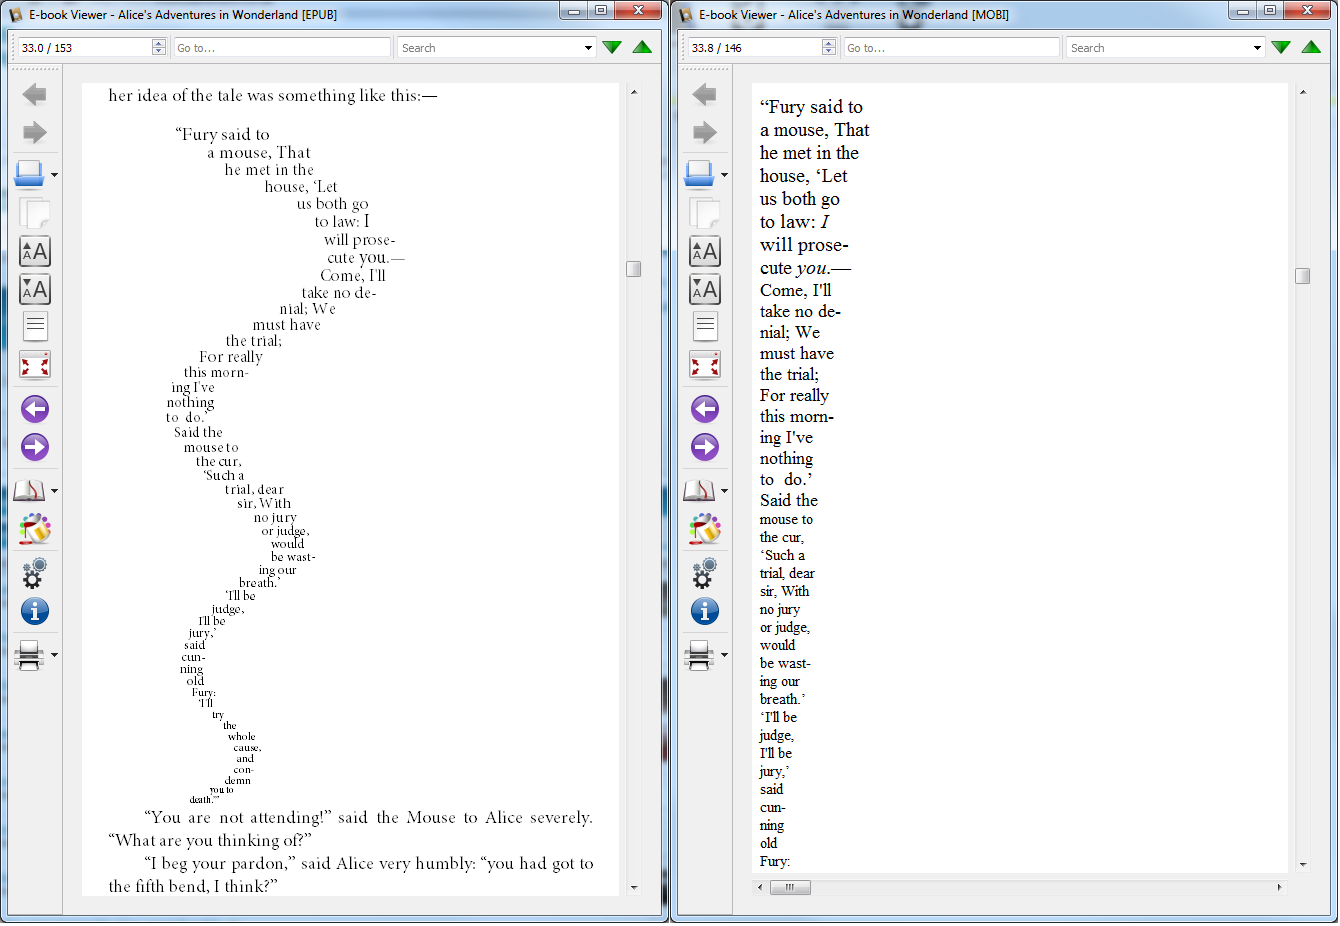
\includegraphics[width=\textwidth]{gfx/alices1}
\caption[Document displayed in Calibre]{On the left is
an \epub{} version of Alice in Wonderland, displayed in Calibre (an open source desktop \ebook{}
viewer). On the right is the same file, converted to Mobipocket, also displayed in Calibre. Note
that in addition to the indentation being lost, the (embedded) font from the \epub{} is no longer
present in the Mobipocket file.}
\label{alices1}
\end{figure}

\marginpar{Mobipocket\ed can't embed fonts... very limited choice of html to use. Reliant on
rendering engine of device.
\epub{}\ed can embed fonts, can style with \css{} pretty much arbitrarily, but still needs to be
retypeset on each viewing and thus relies on the crappy built in rendering engine of the device.}

\epub{} is a little more flexible, in that it supports a more comprehensive range of \xhtml{} and
\css{}, and allows for arbitrarily complex styling. \epub{} files are still entirely reliant on the
rendering engine of the display device correctly displaying their content, as they have no concrete
layout associated with them.

\begin{figure}[tb]
\begin{center}
\vspace{-.3in}
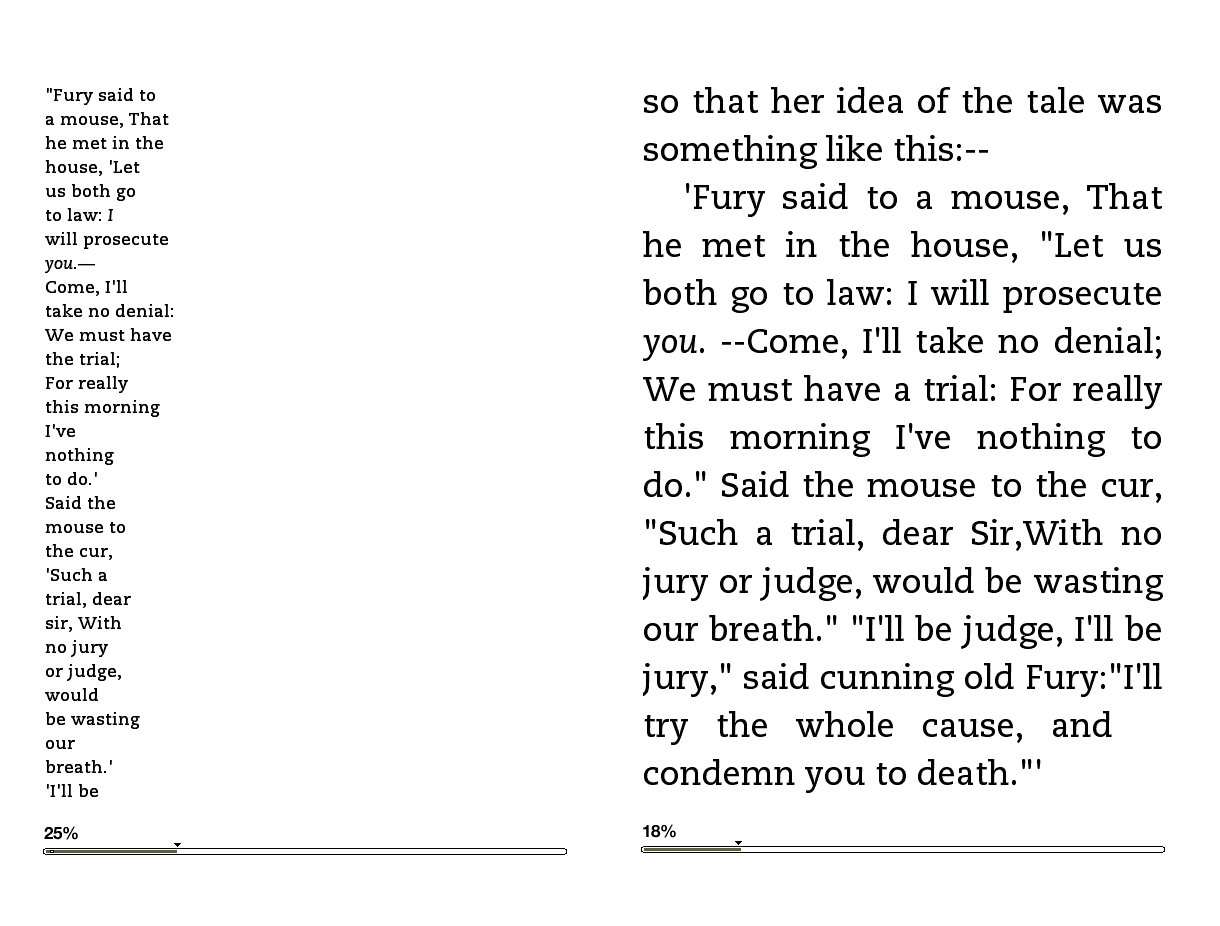
\includegraphics[width=\textwidth]{gfx/alices2}
\end{center}
\vspace{-.3in}
\caption[The same document displayed on the Kindle]{On
the left is the Mobipocket version of Alice in Wonderland (from figure~\ref{alices1}) displayed on
the Kindle. Note that the sizing instructions appear to have been ignored. On the right is the free
version of Alice in Wonderland from the Kindle store, displayed on the Kindle. Note that no attempt
has been made to render the poem in a `tail' shape.}
\label{alices2}
\end{figure}

\section{``Good'' typesetting}
\label{goodtypesetting}
The paper \emph{Reflowable Documents Composed From Pre-rendered Atomic Components}\cite{Pinkney2011}
(attached as an appendix) goes into some detail, particularly in sections 2.1 and 2.2, of what sort
of properties to expect from good-quality typesetting.

Knuth and Plass's line breaking algorithm\cite{Knuth1981}, in conjunction with Liang's hyphenation
algorithm\cite{Liang1983}, breaks paragraphs into lines of text to fit a page, into what can be
considered to be an optimal configuration. \TeX 's default behaviour is then to alter the spacing
between words in order to justify the line to fit the measure of the page. More advanced methods
than simply stretching or shrinking the word spacing do exist, however. Robert Bringhurst, in
\emph{The Elements of Typographic Style}\cite{Bringhurst2008}, suggests that in additon to altering
word spacing, subtle changes to inter-character spacing and individual glyph widths (in the range of
$\pm$ 3\%) can produce more typographically and aesthetically pleasing results. This is discussed
further in section~\ref{edgecases}.

\marginpar{H+J. What is good H+J? Good hyphenation algorithm. Word spacing. Letter spacing. Glyph
reshaping. Must look at whole paragraph!}

\marginpar{Use of kerning. Use of ligatures where appropriate. Avoidance of widows/orphans.}



\cleardoublepage
\chapter{The Malleable Document}\label{ch:malleable}  % ``Aims \& objectives''?? Booooring
%The real aim of this project is to produce documents that are adaptable to multiple viewing
%apertures, but do not require total reprocessing to do so.

%Chapter~\ref{ch:intro} goes into considerable detail
%about precisely which elements of a typeset document must be considered
%computation-heavy (and thus should be avoided if possible at view-time).
%This chapter goes some way towards defining exactly which portions of the
%typesetting process can be pre-computed and which cannot. It also analyses where shortcuts
%can be taken, and their effects on the final document.

\section{The use of Galleys in Typesetting}
The invention of movable type in China in the 11th Century, and independently in Europe in the 15th Century, led to an enormous increase in the availability of printed material. Movable type, in various incarnations, formed an enormously important part of the newspaper industry, from its advent in the 17th century until digitisation in the mid-1980s. The inherently volatile nature of newspaper layout (caused, for example, by important stories breaking shortly before going to press) coupled with the expense and time-consuming nature of physical typesetting, led to the development of the familiar columnar appearance of the newspaper that is prevalent worldwide.

In a traditional newspaper layout, each page is divided into columns of equal \emph{measure}, that is of equal horizontal width. All text to appear in the newspaper is typeset to fit this measure (or integer multiples thereof, for example in the case of headlines) allowing articles to be slotted anywhere into the final layout of the newspaper, simply by breaking their text between lines where necessary to span across columns or pages. The article never requires retypesetting as long as its content remains unchanged\ed{}an advantage only available when all text is rendered to the same width.


The metal trays used to contain typeset lines of physical type are known as \emph{galleys}. Newspapers use reasonably narrow galleys; paperback books tend to use wider galleys, and hardback books wider still.\marginpar{A very unscientific survey of various items of print around my desk suggests that newspapers use approximately 2'' galleys, paperback books around 4'', and hardback books around 5''.} Narrower galleys offer the advantage that less space is wasted if the final line in a paragraph does not span the full width: this is more important in newspaper layout than in most other typesetting situations, as space is at a premium. Wider galleys aid readability, up to a certain point, after which it becomes difficult for the eyes to keep track between lines.\cite{Bringhurst2008, Voorhees2011}


Typesetting text into physical galleys is directly analogous to precomputing many of the `hard' parts of typesetting. In particular, all hyphenation, line breaking, justification, kerning, glyph substitution etc.\ed{}in fact all horizontal layout\ed{}has been `compiled out'. No matter the height of the page nor the number of columns, only vertical layout problems remain, such as attempting to avoid widowed or orphaned lines, and choosing optimal placements of floating bodies, such as pictures or figures.

\section{Galleys as a Reflow Tool}
If an electronic, primarily text-based document can be partially pre-rendered into the analogue of a galley, the document is then provided with some limited flowability. Specifically, the document can be rendered for any page size at least as wide as the galley, and of arbitrary height. Wider pages may be able to accommodate multiple columns, but unless the page size is chosen carefully based on the galley's width, there is likely to be noticeable extra horizontal whitespace if the page width is not close to a multiple of the galley width.

\begin{figure}
 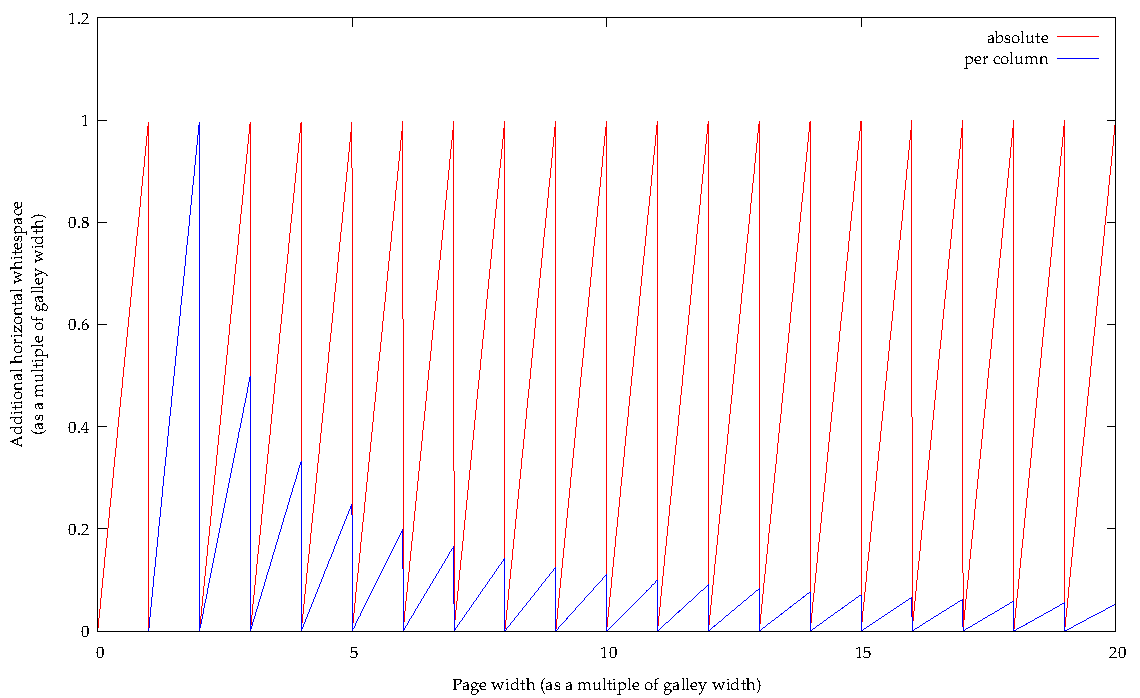
\includegraphics[width=\textwidth]{gnuplot/1col}
 \caption[Extra whitespace in a single-galley document]{As more columns fit on a page, the extra whitespace required per column decreases}
 \label{fig:sawtooth}
\end{figure}


Figure~\ref{fig:sawtooth} shows how the extra horizontal whitespace on a page varies with page width. The peaks are at the point where an extra column can be added, and the amount of extra whitespace required drops to a minimum. The green dashed line divides this extra whitespace by the number of columns on the page, which gives a more useful metric to work with: if we physically divide the extra whitespace and insert it between the columns to increase their spacing (as opposed to leaving it on the right- or left-hand margins) then the wider the page, the less detriment is caused by the extra fraction of galley width.

\section{Multiple Galley Renderings}
The problem of extra whitespace can be overcome in several ways. Firstly, and most simply, the scaling of the galley can be altered, effectively simulating a change in the point size of the font. This is probably undesirable unless a change in point size has explicitly been requested, especially if any size change is particularly noticeable.
A second way in which columns can be better fitted to the page width is to typeset the source document into a range  galleys of varying width. When the document is rendered at view-time, the most appropriate width (according to some metric) can be chosen to be displayed. One very simplistic metric is to choose whichever galley rendering would result in the least extra added whitespace. By overlaying the Figure \ref{fig:sawtooth}-like graphs for each galley, we are able to obtain a graph like Figure~\ref{fig:overlay}, which features all available galleys. If we use our simple metric of minimum whitespace, we can simply choose whichever galley requires the smallest amount of extra whitespace for a given page width.

\begin{figure}
 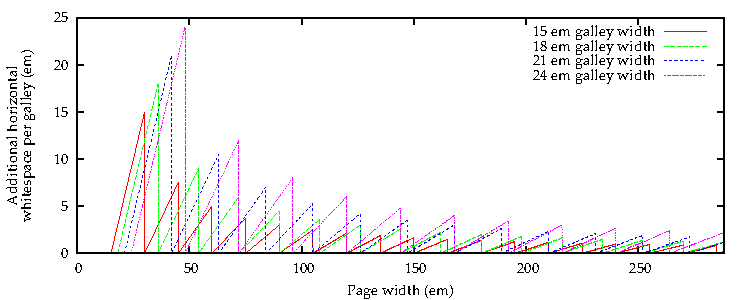
\includegraphics[width=\textwidth]{gnuplot/overlay}
 \caption[Extra whitespace in a multiple galley document]{Overlaying the sawtooth graphs for several galleys of differing widths allows us to minimise the extra added whitespace}
 \label{fig:overlay}
\end{figure}

\section{A Simple Implementation}
At an early stage it was decided that the simplest available method of implementing the above-mentioned layout algorithm was to use some of the University of Nottingham Document Engineering Laboratory's existing tools: in particular the Component Object Graphic (\COG{}) model\cite{Bagley2003} for creating and managing modularised \pdf{} documents. This was chosen specifically to avoid the need to write a typesetter or layout engine from scratch; typesetting is performed by the \troff{} suite, and layout by Adobe Acrobat, though there is no reason why this algorithm could not be implemented with any other system capable of tightly specifying page imaging operations. Indeed, for this to be implemented in any non-prototypal form, \ie{} to be used on any portable device, it is likely that a specific, new rendering engine will need to be written for each device.

\subsection{The Source Document}
Since the majority of available tools for producing \COG{}ged \pdf{}s rely on the typesetting package \ditroff{}, it was decided to use this as the basis for the source document. \Ditroff{} is particularly amenable to many of the features required here\ed{}it is quite happy to have its page length set to large numbers\ed{}one sample document used a page length of 2000 inches (approximately 50 metres) with no complaints from \ditroff{}. The line length was set to a small value (approximately two inches) in order to produce a narrow column of text. Following this, the actual document content was inserted several times, and the line length incremented, producing one document effectively containing multiple galley renderings of the same content.

\subsection{pdfdit}
Having generated the source document, it was processed with ditroff to generate the intermediate code used to feed each typesetter post-pro\-cessor. This output is very expressive, and, unlike \TeX's DVI, contains enough information that post-processors are easily able to locate the start and end of lines and paragraphs within the document. This meant that only minimal changes were needed to be made to the \emph{pdfdit} package described in \cite{Bagley2003} to implement our design.

The first change necessary was to decrease the granularity of the output COGs, producing them at the line level, rather than at the paragraph level. Secondly, some method of generating the requisite tree representing the document structure was required. This was solved by simply using the point at which the original version of pdfdit would have started a new paragraph-level COG, and, instead, starting a new paragraph-level block entry in the document structure tree. Each subsequent line-level COG produced can then be added as a child of this block.

Once the entire output file has been parsed, the tree representations of the various width galleys are amalgamated per-paragraph, as indicated in figure~\ref{tree}, and finally the PDF file is serialised, replete with COGs and content tree.

\subsection{Acrobat Plugin}



\section{Layout Considerations}
eg what sort of layouts are we constricted to, and are they any good... cite Plass/Bringhurst

\section{Efficiency}
theoretically, how does it compare? Shove in lots of speculative Big Oh notation and try to sound authoritative. Or look at the algorithms used and
actually be authoritative :)



% \marginpar{Can we have one physical representation which fits to all devices \emph{and} is
% efficient? Should we perform some pre-processing to the document to tailor it to a particular
% device?}
% 
% Amazon's Kindle Store model provides a good example of the need for multipurpose documents\ed one
% purchase may be viewed on any number of platforms\ed the desktop app, the mobile phone app, the
% tablet app, and on the Kindle itself. Amazon does not currently provide any special dispensation for
% any of the platforms it supports\ed every one receives the same source document to display.
% Consequently, a Kindle book is effectively a jack of all trades, and master of none: instead of
% looking good on any one platform, the books look mediocre on \emph{every} platform. The real
% questions here are as follows:
% 
% \begin{itemize}
%  \item Is it possible to have one physical representation which typesets well on \emph{all}
% platforms whilst remaining efficient enough not to cause excessive battery drain?
%  \item Is it possible to identify invariant features common to many renderings to reduce the need
% for processing on the display device?
%  \item Should a more abstract, higher level of document be provided from which lower-level
% device-specific derivatives can be produced?
% \end{itemize}
%   
% The desire is to develop some document format which is neither as `solid' as a \pdf{} nor as
% `liquid' as \html{}, but somewhere in between (perhaps termed a \emph{malleable document}).
% Something which is mostly formed, but can be gently massaged to fit the display as necessary.
% 
% 
% \section{A Simple Implemenation}
% 
% 
% \marginpar{Mention paper here \cite{Pinkney2011}\ed appendix. Give brief overview of current
% system.}
% The majority of the work to date on this project is described in the paper \emph{Reflowable
% Documents Composed from Pre-rendered Atomic Components}\cite{Pinkney2011}, which was published and
% presented at the 2011 ACM Symposium on Document Engineering. It is also attached to this document as
% an appendix.
% 
% The paper outlines a very simple approach towards a malleable document format: the source document
% is simply rendered into `galleys' of text (see \cite{Pinkney2011}, section 3) multiple times, using
% a high-quality typesetting algorithm, with each rendering using a different galley width. The
% document is thus now displayable on multiple screen sizes (each width rendering may additionally be
% scaled by the display device to simulate point-size changes) without the need for the document to be
% expensively retypeset. The `best fit' rendering is chosen at display time, based on the available
% screen width and zoom level. The current implementation of this system is built around pre-existing
% tools for the \emph{ditroff} typesetting system\cite{Kernighan1982} and Component Object Graphic
% PDF\cite{Bagley2003}.
% 
% \subsection{Efficiency}
% \marginpar{Computational\cite{Knuth1981} \& space.}
% It is clear that computational efficiency must be maximised in order to minimise processor usage and
% battery drain. In order to do this, it will almost certainly be necessary to sacrifice storage
% efficiency; that is, filesizes are likely to be bigger. This is not necessarily a problem. Storage
% is cheap and plentiful; currently it is far more practical and cost effective to increase storage
% space than battery life. For this reason, we shall not concern ourselves too much with producing
% documents with small filesizes, and shall instead concentrate on pre-computing as much of the
% typesetting as possible, whilst retaining flexibility.
% 
% \subsection{Handling of edge cases}
% \label{edgecases}
% \marginpar{Corner cutting? Adjusting spacing\ldots word/letter spacing, glyph reshaping.
% \cite{Bringhurst2008}}
% The work described in \cite{Pinkney2011} and outlined above does not contain any special handling
% for edge cases, although this will not be difficult to implement. In particular, the system is
% currently restricted to displaying text only in the exact manner in which it was rendered. As an
% example, let us assume that a particular point size has been selected (i.e.\ the zoom level has been
% fixed); the best fit galley is then chosen for the page width. It may be the case that this
% particular galley rendering, at this zoom level, on a page of this width results in large margins.
% Perhaps the next galley size up is too wide to display. Currently, the penalty is simply to have to
% put up with these large margins. However, there are some simple tweaks which can be used to reduce
% how noticeable this effect is. As stated in section~\ref{goodtypesetting}, whilst performing
% justification, it is occasionally appropriate to adjust letter spacing and glyph widths, in addition
% to word spacing. Whilst readjusting these three
% parameters \emph{after} justification has taken place may reduce the typesetting quality (by making
% any of them larger or smaller than allowed by the justification rules) in certain cases it may be
% acceptable to do so, to fit the pre-rendered galley lines to a different width. Using the current
% implementation, it is particularly simple to adjust the word spacing\ed in the PDFs produced, each
% word is stored distinctly, and so can be repositioned as necessary. It is also very simple to
% reshape the glyphs, to either stretch or shrink them laterally. All PDF drawing operators are
% executed in accordance with the current \emph{transformation matrix}, which alters the coordinate
% system\cite{Adobe2001}. Glyph reshaping can thus easily be performed on any word or line by altering
% this before calling the requisite drawing operator. It is more difficult to alter the letter
% spacing, particularly in the current implementation, as this will involve looking up font metrics,
% and will be comparatively inefficient.
% 
% 
% \subsection{Examples of these principles in practice}
% Of particular interest and relevance to this thesis, is Amazon's recently announced Silk web browser
% for their new Kindle Fire platform. Silk uses a similar paradigm to that outlined in
% \cite{Pinkney2011} in order to serve web pages to the Kindle Fire, in a manner that requires less
% processing by the device itself. Amazon makes use of its extensive computing power in its Cloud
% service to prerender any webpage requested through Silk. The output is tailored specifically to the
% device, enabling, for instance, layout of tables, or image scaling, to be performed on the Cloud
% servers rather than locally on the device. Amazon has produced a five minute technical overview
% video, available at \verb+http://www.youtube.com/watch?v=_u7F_56WhHk+
% 
% 
% \subsection{Anticipated extensions}
% \marginpar{Newspaper galley creation guidelines? look into\ldots}
% Since the current work relies heavily on the setting of text into galleys, it would probably be
% pertinent to research newspaper galley creation guidelines. These may be difficult to come by, since
% newspapers have been electronically typeset for much of the last three decades. Nevertheless, the
% information must be available somewhere, and could prove invaluable.
% 
% \marginpar{Device profiles\ldots what is appropriate? Image resolution? Page width renderings for
% specific screen size?}
% At some point, it will probably prove necessary to tailor the output document to the specific device
% for which it is intended. Accordingly, profiles for these devices must be devised, which contain all
% the necessary attributes to produce a document to fit. For example, image resolution must be
% considered. Is there a necessity to use hi-resolution images for a document which is to be displayed
% on a mobile phone screen? Perhaps not. Whilst a large image may be scaled down to fit, unless the
% image is required to be zoomable, it seems sensible to precompute this scaling, and remove the need
% for the device to perform it each time the image is displayed. Similarly, it may be sensible to
% generate galleys only in sizes appropriate to the device. A mobile phone is clearly going to require
% narrower renderings than a tablet, for example. Whilst each document \emph{could} include many
% resolutions of each image, and a vast range of galley width renderings suitable for many devices, it
% seems rather wasteful to do so when
% these tailored versions can easily be produced. It is envisaged that such a system would run on a
% user's desktop or laptop PC, which would store the canonical, high-level representation of the
% document, and that the apparent copying of that document to a display device would in fact create a
% bespoke version of the document, specifically to fit the device, yet still with enough flexibility
% to allow the font size to be changed within sensible limits.
% 
% \marginpar{Perhaps suggest using vector images where possible?}
% 
% 
% \subsection{Conclusions}
% \marginpar{Need to balance time/complexity against appearance. Comparable to eg Plass/Knuth? thus
% need some way to quantify appearance\ed some form of metrics needed for this. Needs
% investigation\ldots}
% Computational efficiency is easily quantifiable, both on a theoretical level, and experimentally.
% Typesetting quality, however, is harder to quantify. In order to show whether this system can
% produce consistently better results than a standard \ebook{} layout engine, some method must be
% derived in order to compare them. This may be based on a point-scoring system, in a similar manner
% to \TeX{}\cite{Knuth1984}, or perhaps by more qualitative means, such as human judgement. In either
% case, both these factors must be balanced against one another, striving to reduce computational
% efficiency whilst maintaining typesetting quality.
% 
% 
% 
% 
% 
% \section{Introduction}
% In recent years, the consumption of documents on mobile devices, such as eBook readers, has
% increased dramatically. However, the visual quality of a document on these devices is often lacking,
% when compared to other digital document systems (see figure \ref{kindle}). The result of an eBook
% reader's layout engine is often visually unappealing, with uneven spacing in consecutive lines of
% text, poor justification, and the lack of a sophisticated hyphenation system.
% 
% This is a far cry from the quality of typesetting available from PDF or PostScript documents. These
% vector-based, de\-vice-in\-de\-pen\-d\-ent page description languages are able to create a digital
% version of the document that is identical to its printed counterpart. These page description
% languages, coupled with high-quality typesetting systems (such as \TeX{}, troff or Adobe InDesign)
% have produced an expectation that digital documents will be of similar quality to that achievable
% through hand composition. \TeX{} and Adobe InDesign, in particular, have excellent support for many
% of the subtle nuances used by hand compositors, which are often overlooked by more basic typesetting
% packages (e.g.~automated support for kerning and ligatures). This quality does not come without a
% price: the algorithms used to calculate the layout are computationally expensive and so are run only
% once, to produce a PDF with a fixed layout targeted at a fixed page size.
% 
% eBook readers, it seems, have had to take a step backwards to simpler (and, therefore, less
% computationally expensive) algorithms to maximise the battery life of the device. The result is that
% the high-end hyphenation, kerning, and ligature support has had to be sacrificed and the on-screen
% result is reminiscent of the output of an HTML rendering engine or a very basic word processor.
% 
% This paper investigates an alternative approach to generating the display for an eBook reader. Here,
% the text is pre-rendered (using a high-quality typesetting algorithm) in several column widths,
% prior to display, when the document is created. At view time, the most appropriate column width is
% selected for display, the system balancing between excessive white space and multiple columns.
% Section~\ref{problems} examines the problems posed by current eBook readers in further detail, while
% section~\ref{solution} presents our initial prototype solution to some of these problems.
% 
% \section{Problems with Current eBook Readers}
% \label{problems}
% Three formats currently dominate the eBook market: EPUB and Mobipocket, which allow the document to
% be formatted to fit the device, and PDF, which does not. (Amazon's proprietary Kindle format is
% derived from Mobipocket; PDF and EPUB are open standards.) Both the EPUB and Mobipocket formats are
% largely based on XHTML. Whilst the use of XML-derived formats allow the semantic structure of
% documents to be very well defined, in general their presentation can only be specified in a very
% loose manner. The user is often presented with a choice of typefaces and point sizes, allowing the
% reader software to render the document in essentially any arbitrary way it chooses.
% 
% Conversely, PDF is entirely presentation-oriented, stemming from its origin of being compiled
% PostScript. PDF, therefore, will often include no information on the semantic structure of the
% document, and will consist simply of drawing operators which describe the document pages. There is
% no compulsion for these drawing operators to render the page in an order that might be considered
% sensible: for example, if a PDF generator program decided to render every character on a page in
% alphabetical order, or radially outwards from the centre, the resulting file would still be
% semantically valid, and the result might well be unnoticeable to the end user. This lack of imposed
% semantic structure can make it difficult to infer the best way to `unpick' PDF files to allow their
% content to be reflowed into a new layout.
% 
% Since an XHTML-derived format has no fixed presentation associated with it, this must be calculated
% each time the document is displayed, in a similar manner to the way an interpreted programming
% language needs to be interpreted each time it runs. For an eBook reader to maximise its battery life
% (the human reader will be annoyed if the device dies just before the climax of a novel!), the
% `interpretation' needs to be as simple as possible\,---\,i.e.~the algorithm used must not be too
% complex, since the more CPU cycles spent executing it, the less time the CPU can spend idle, and
% hence the greater the drain on the battery. Furthermore, the longer that is spent formatting the
% output, the longer the delay between page turns on the device, and with the speed of CPUs used in
% these devices (<~500~MHz) it does not take too large an increase in computation for the page turn to
% become noticeable.
% 
% \begin{figure}
%     \centering
%     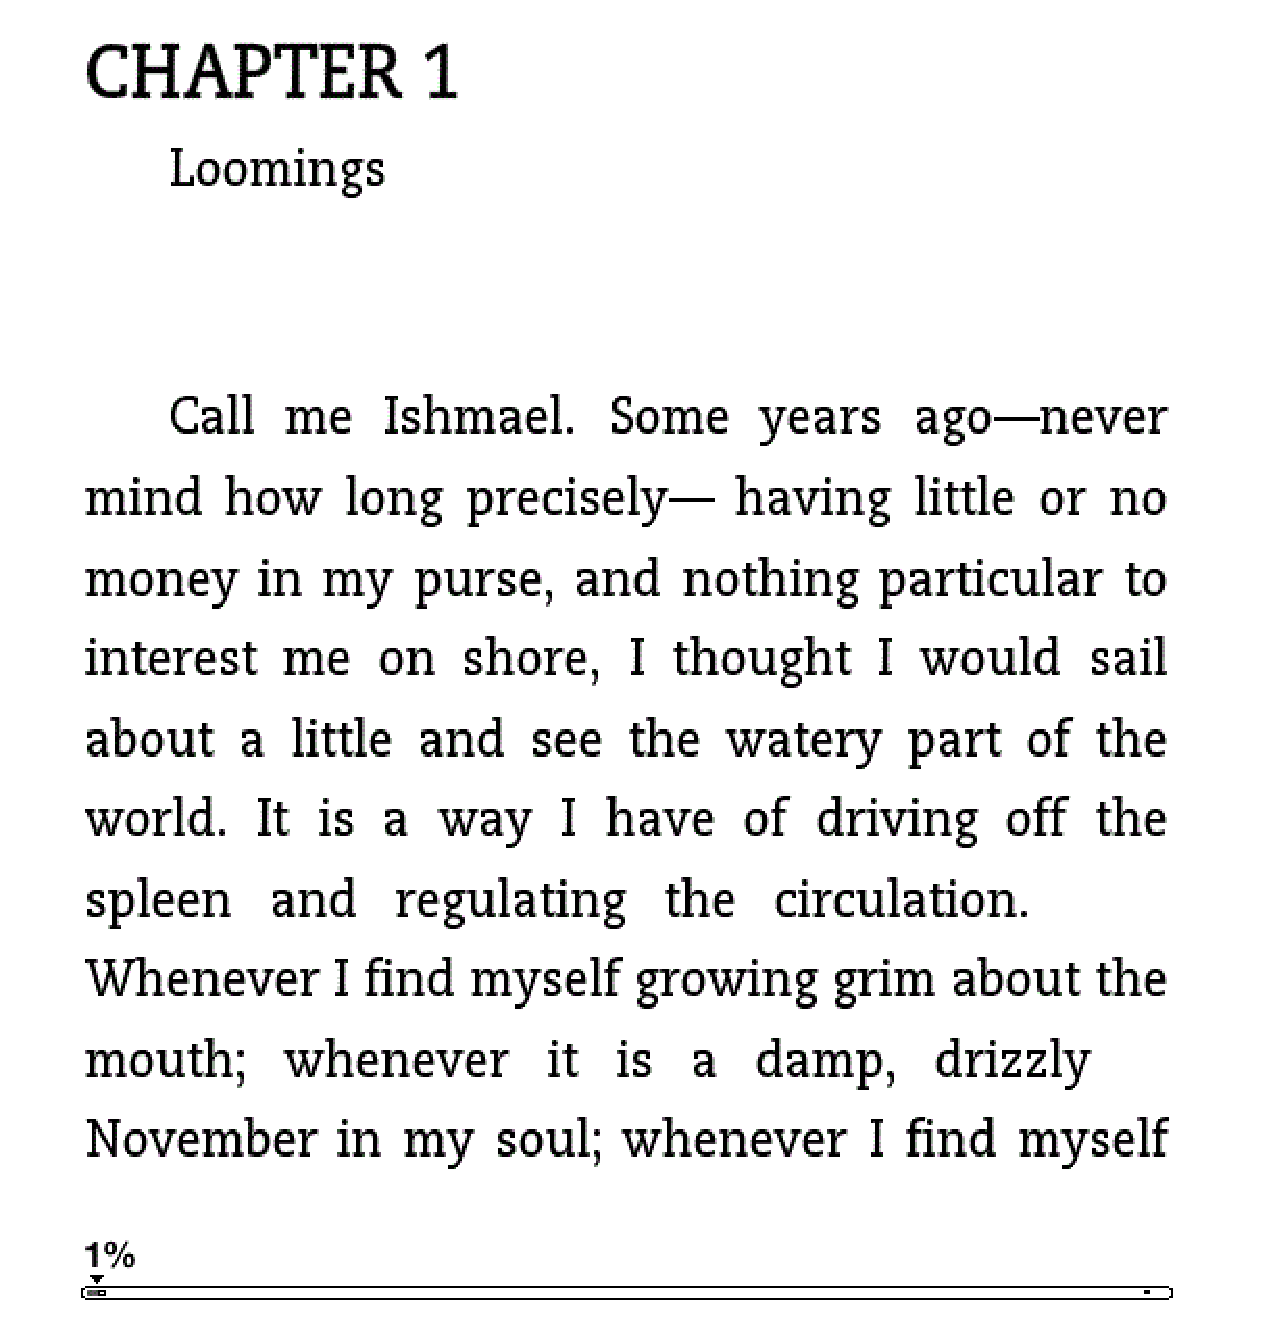
\includegraphics[width=\textwidth]{gfx/screen_shot-42583}
%     \caption[An example of typesetting on the Kindle]{The Kindle 3 appears to primarily use
% justified text, falling back to ragged-right when
% inter-word spacing would become too large.}
%     \label{kindle}
% \end{figure}
% 
% \subsection{Hyphenation and Line-Breaking}
% eBook readers typically use a `greedy' algorithm to lay out their text\,---\,that is, they place as
% many words as will fit onto the current line without exceeding it, then start a new line and
% continue. Although this algorithm is optimal in that it will always fit text onto the fewest
% possible lines, it often causes consecutive lines to have wildly varying lengths, accentuating
% either the `ragged-right' effect of the text, or, in the case of justified text, the inter-word
% spacing. In general, eBook readers will only hyphenate in extreme cases\,---\,indeed the Kindle~3
% seems not to do so at all. Knuth and Plass\cite{Knuth1981} developed a more advanced line-breaking
% algorithm (now used by \TeX{}) which attempts to minimise large discrepancies between consecutive
% lines by considering each paragraph as a whole. \TeX{} also uses the hyphenation algorithm designed
% by Liang\cite{Liang1983}, which has been ported to many other applications.
% 
% \subsection{Other Typographical Techniques}
% Other techniques employed during hand-type\-set\-t\-ing and high-qua\-l\-ity electronic typesetting
% include the use of kerning and of ligatures. Kerning involves altering the spacing between certain
% glyph pairs in order to produce more consistent letter spacing, whilst ligatures are sin\-gle-glyph
% replacements for two or more single glyphs which may otherwise have clashing components. Some
% examples of these are shown in figure~\ref{kern-lig}.
% Kerning requires a table of kern-pairs, specific to each font; values from this table must then be
% looked up for every pair of adjacent glyphs in the document. Ligatures may or may not need to be
% inserted: if the component characters of the ligature lie over a potential hyphenation point, it
% cannot be decided whether to replace them with the ligature until it is known whether the
% hyphenation point needs to be used.
% 
% 
% \begin{figure}
% 
%     %\centering
%     \vspace{-24pt}
%     {\Huge \textbf{
%     \begin{tabbing}
%     \hspace{0.1in} \= T\mbox{}o \= A\mbox{}V \= V\mbox{}. \= W\mbox{}a\hspace{0.3in}\= f\mbox{}i \=
% f\mbox{}l\\
%     \> To \> AV \> V. \> Wa \> fi \> fl
%     \end{tabbing}
%     }}
%     \caption[Examples of kerning and ligatures]{Examples of various letter-pairs and their kerned
% (left) or ligature (right)
% equivalents, as typeset by \TeX{}.}\vspace{-3pt}
%     \label{kern-lig}
% \end{figure}
% 
% 
% % % % % % % % % % % % % % % % % % % % % % % % % % % % % % % % % % % % % % % % % % % % % % % % % % %
% 
% 
% \section{A Galley-Based Approach}
% \label{solution}
% %note that storage is \textbf{not} at a premium, but battery life/processor are.
% %Prerender as much as possible, ie at compile-time
% %Layout then becomes simple. Allows arbitrarily complex layout with no overheads at runtime
% %Include a tree so the semantic structure of the document is explicit
% Our proposed solution, of precomputing several text variants, revisits an approach to typesetting
% from before the advent of desktop publishing. In the days before DTP, newspaper articles were
% typeset into long columns known as \emph{galleys}. Since all columns in the newspaper would be of
% uniform width, all articles could be typeset into galleys of the same measure, and then broken as
% necessary between lines, in order to slot into the final layout of the newspaper. Once the text has
% been set in this manner, with appropriate hyphenation and justification, the individual lines can be
% treated as atomic units that will never have to be re-typeset. In essence, each article is
% `compiled' only once, but can be used anywhere in the final layout without penalty.
% 
% %could this all be one paragraph?
% 
% It is this behaviour we wish to emulate. So long as the atomic components of the document are
% tightly specified, and the reader software can obey the associated drawing instructions (essentially
% treating them as pre-typeset blocks), the resulting display of the document will be of as high
% typographic quality as that of the original galley, and the requirement for further computation will
% be vastly reduced. In order to permit aesthetic layout for a wider range of screen sizes, it seems
% sensible to create a document containing multiple renderings of the same content, and simply
% choosing the `best fit' rendering when the document is displayed.
% 
% %Something about ideal text measure\cite{Bringhurst2008}
% 
% %need to say several renderings included
% 
% 
% \subsection{A Sample Implementation}
% Our sample implementation is built around our existing work in PDF and Component-Object Graphics
% (COGs)\cite{Bagley2003}, but there is no reason why it could not be implemented in any other format
% capable of tightly specifying page imaging operations. It builds on existing software, principally
% \emph{pdfdit}, in conjunction with \emph{COG Manipulator}, as these tools are already capable of
% producing modular documents with tightly specified rendering.
% 
% 
% \subsubsection{The COG Model}
% %summary of cogs, what I've changed, ie line-level rather than default paragraph level. Put in tree
% to retain par details
% The Component Object Graphic (COG) model was developed to enable the reuse of semantic components
% within PDF documents, by breaking the traditional graphically-monolithic PDF page into a series of
% distinct, encapsulated graphical blocks, termed COGs. In its original incarnation, the COG model did
% not account for any relationship between individual COGs\,---\,it was simply designed as a method by
% which document components could be easily reused or reordered. The COGs it generates are largely at
% the granularity of a paragraph, and can still be imaged onto the page in any arbitrary order,
% independent of reading order.
% 
% In order to implement our galley-based design, it is necessary to decrease this granularity, such
% that each line of text is represented by a separate COG. However, it is also important that the
% semantic structure of the document is explicitly stored. This is principally so that the reading
% order of the COGs is maintained, and also so that the reader software can identify paragraphs,
% headings etc.~to enable them to be laid out correctly.
% 
% The COG model takes advantage of the fact that the PDF specification allows the content of a page to
% be described by an array of streams of imaging operators, rather than the more commonly encountered
% single, monolithic stream. Unfortunately, this array can only be one-di\-men\-sional, meaning that
% while it can enforce the reading order, it cannot be used to, say, group lines into paragraphs.
% Since the PDF specification allows essentially arbitrary insertion of data structures into a
% document (PDF readers which do not recognise these will simply ignore them), this flexibility was
% used to embed a simple tree structure representing the paragraphs, in parallel to the COGs
% themselves (an example of which is shown in figure~\ref{tree}). At the level of its leaves, this
% tree simply contains pointers to the COGs which make up the content of the document. In the simplest
% case, where the document contains only one rendering (and thus the pa\-ra\-graph-level items have
% only one child) the COGs pointed at by the leaves can simply be rendered in order, adding vertical
% space as appropriate.
% 
% 
% \begin{figure}
%     \centering
%     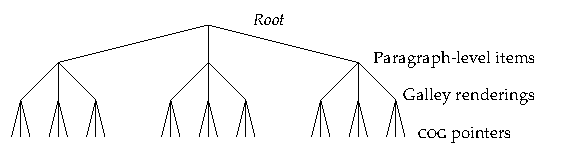
\includegraphics[width=\textwidth]{gfx/tree}
%     \caption[A simple document structure tree]{A simple document structure tree. The first level
% below the root represents all
% paragraph-level items: headings, paragraphs, figures etc. These items have one child for each galley
% rendering of the document. These in turn have one child for each COG comprising their
% content\,---\,in the case of a paragraph or heading: its lines; in the case of a figure: the figure
% itself and any associated caption.}\vspace{-3pt}
%     \label{tree}
% \end{figure}
% 
% \subsubsection{The Source Document}
% Since the majority of available tools for producing COGged PDFs rely on the typesetting package
% \emph{ditroff}, it was decided to use this as the basis for the source document. Ditroff is
% particularly amenable to many of the features required here\,---\,it is quite happy to have its page
% length set to large numbers\,---\,one sample document used a page length of 2000 inches
% (approximately 50 metres) with no complaints from ditroff. The line length was set to a small value
% (approximately two inches) in order to produce a narrow column of text. Following this, the actual
% document content was inserted several times, and the line length incremented, producing one document
% effectively containing multiple galley renderings of the same content.
% 
% 
% %- troff source doc, long page, narrow column, creating galley
% 
% \subsubsection{pdfdit}
% Having generated the source document, it was processed with ditroff to generate the intermediate
% code used to feed each typesetter post-pro\-cessor. This output is very expressive, and, unlike
% \TeX's DVI, contains enough information that post-processors are easily able to locate the start and
% end of lines and paragraphs within the document. This meant that only minimal changes were needed to
% be made to the \emph{pdfdit} package described in \cite{Bagley2003} to implement our design.
% 
% The first change necessary was to decrease the granularity of the output COGs, producing them at the
% line level, rather than at the paragraph level. Secondly, some method of generating the requisite
% tree representing the document structure was required. This was solved by simply using the point at
% which the original version of pdfdit would have started a new paragraph-level COG, and, instead,
% starting a new paragraph-level block entry in the document structure tree. Each subsequent
% line-level COG produced can then be added as a child of this block.
% 
% Once the entire output file has been parsed, the tree representations o-f the various width galleys
% are amalgamated per-paragraph, as indicated in figure~\ref{tree}, and finally the PDF file is
% serialised, replete with COGs and content tree.
% 
% 
% %Note also the inclusion of baseline/indent?
% 
% %summary, plus what's changed (similar to the above)
% 
% 
% 
% \subsubsection{Acrobat Plugin}
% \begin{figure}
%  \centering
%  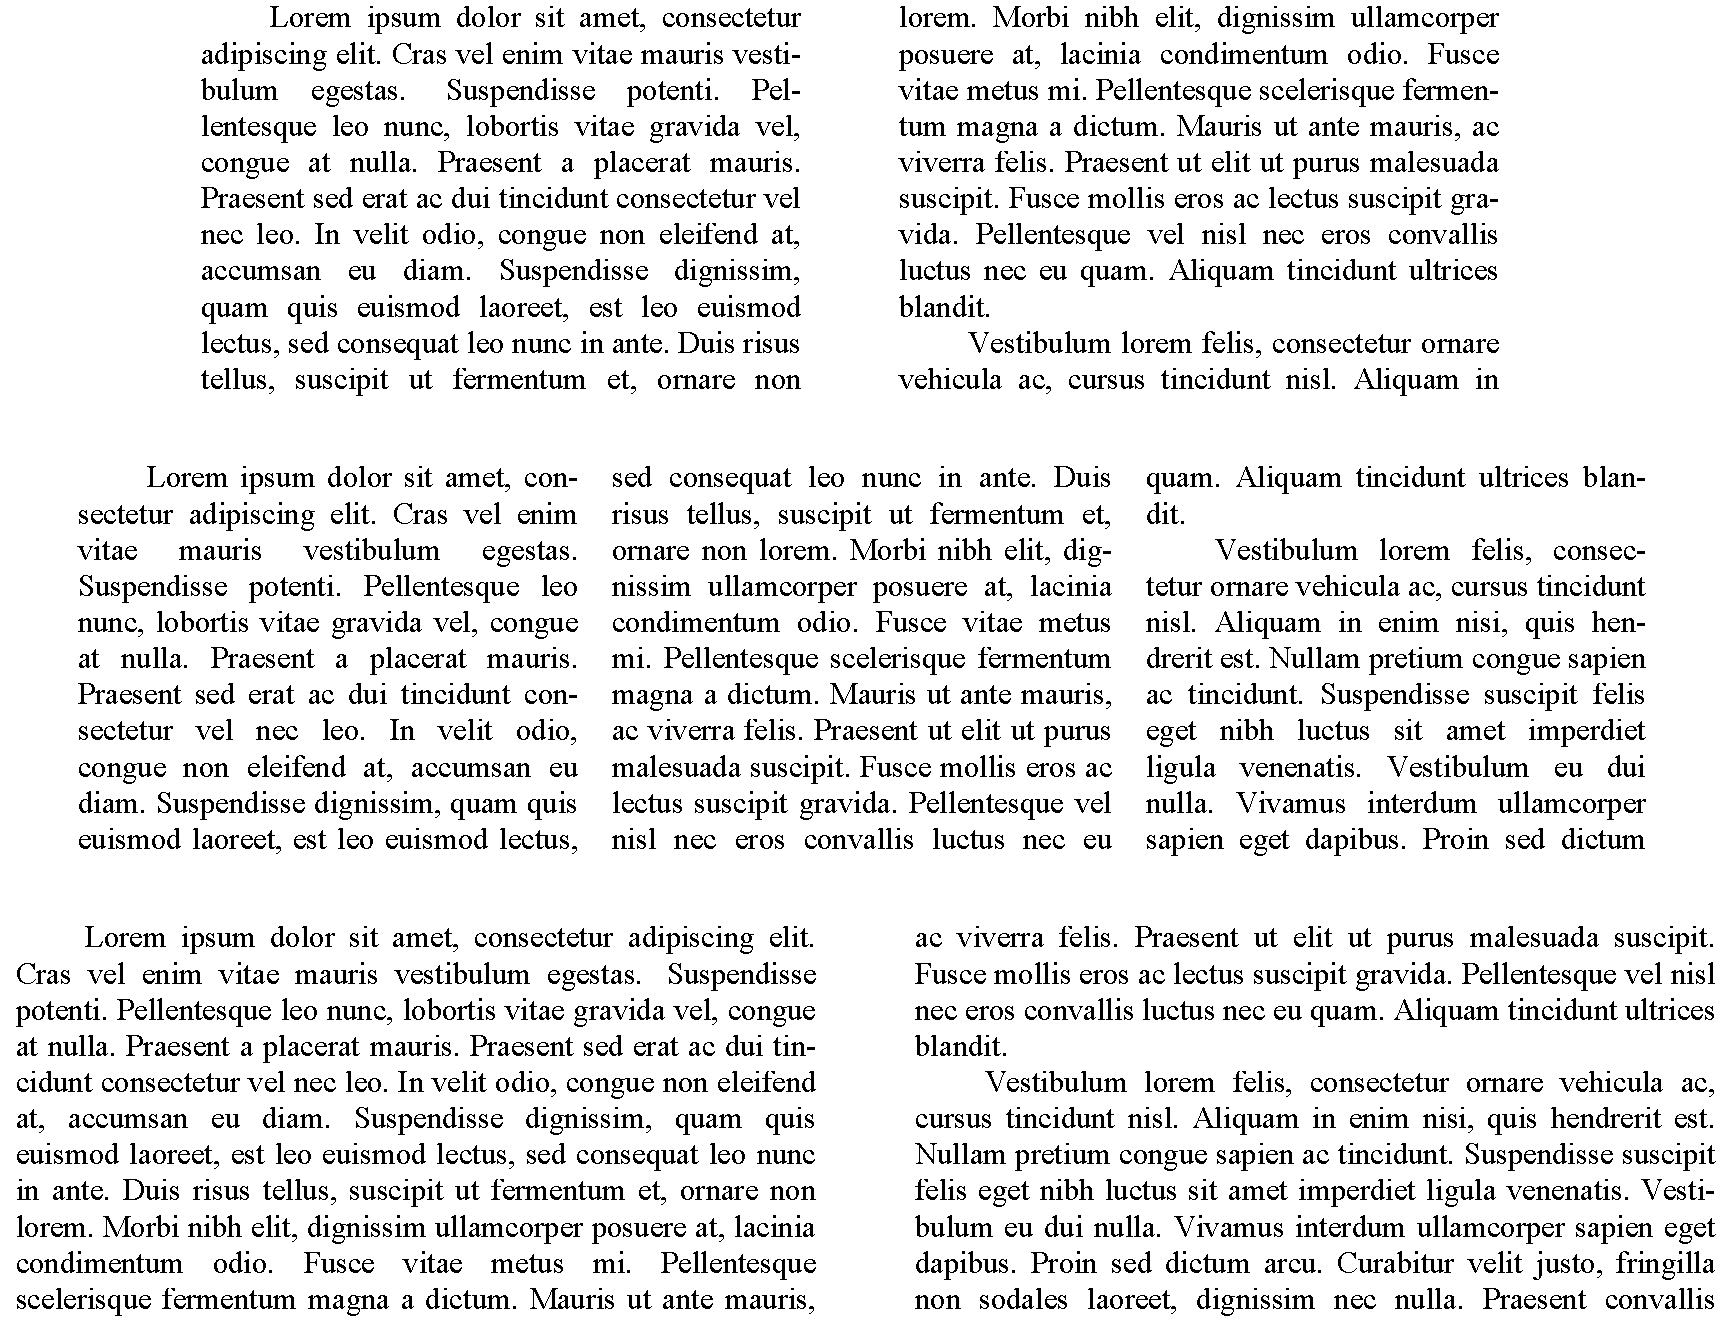
\includegraphics[width=\textwidth]{gfx/renderings}
%  \caption[Sample renderings from the Acrobat plugin]{Sample renderings from the Acrobat plugin at
% page widths of 42, 48, and
% 54~em.}
% \end{figure}
% 
% \begin{figure}
%     \centering
%     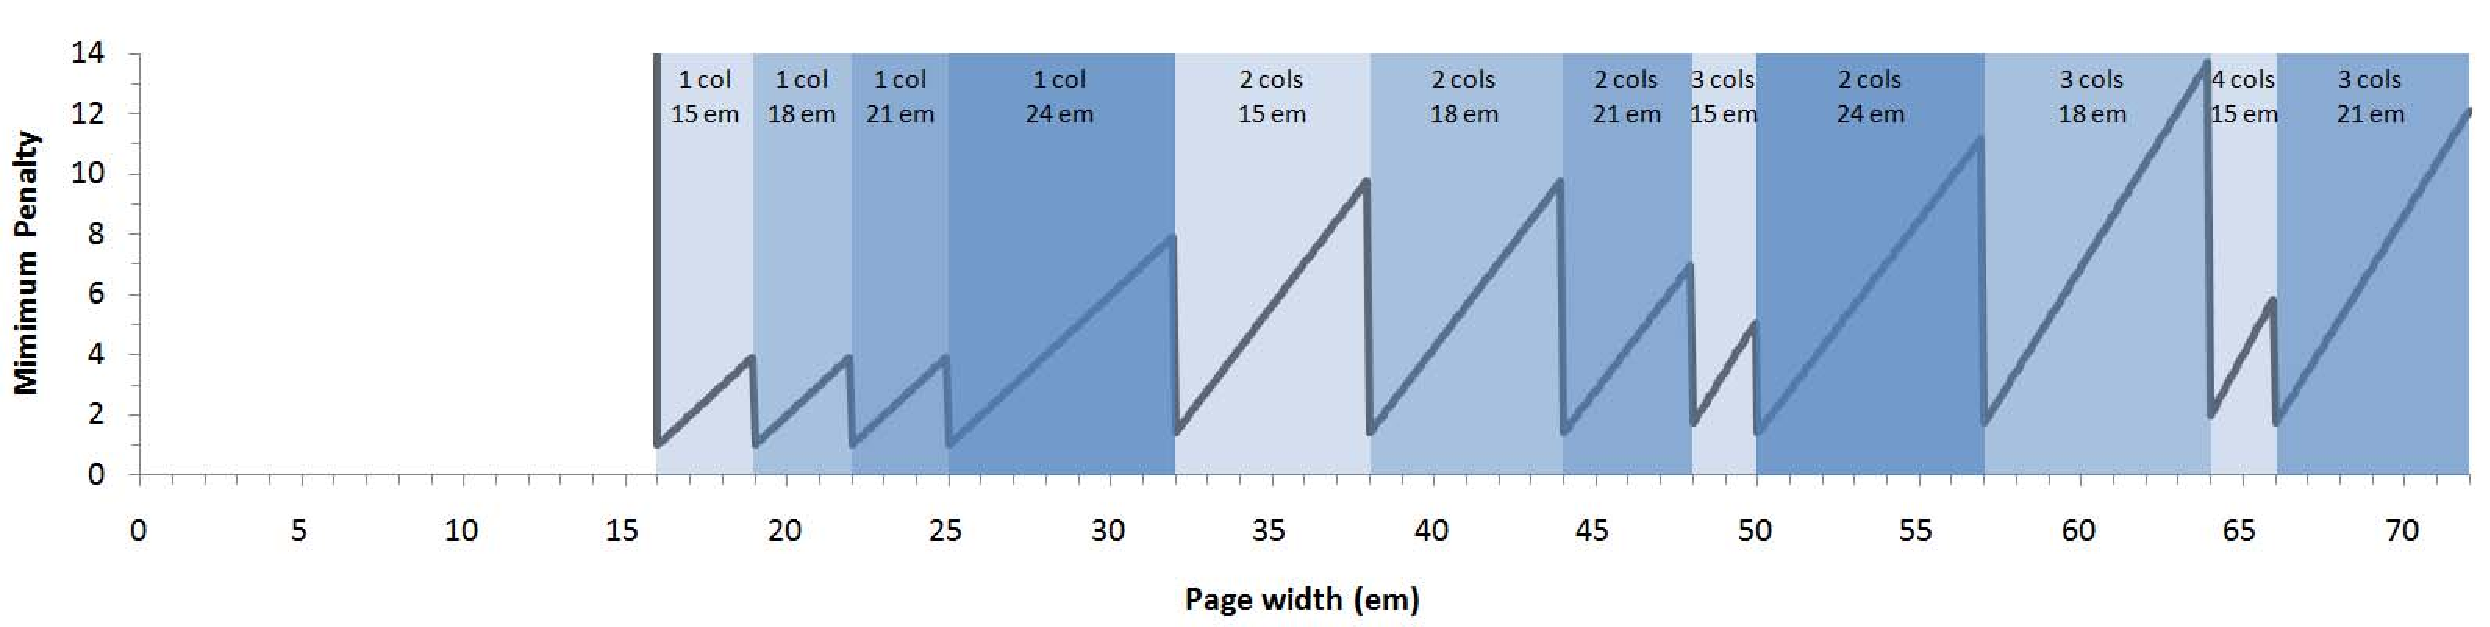
\includegraphics[width=\textwidth]{gfx/graph-em}
%     \caption[Layout Penalty Graph]{Graph showing the minimum penalty value of
% all galleys in a reflowable document, over a
% range of page widths. The particular document used contained four galleys; these were rendered at
% widths of 15, 18, 21 and 24~em, with a minimum gutter width of 1~em. Each vertical band highlights a
% range of page widths within which only the horizontal spacing of the page is altered. The boundaries
% between vertical bands represent a switch between galley renderings\,---\,the galley used and number
% of columns is as annotated on the graph.}\vspace{-3pt}
%     \label{graph}
% \end{figure}
% 
% The decision to use Acrobat as an eBook `emulator' stemmed once again from the available existing
% COG-based tools, as well as the extensive API and developer support available for Acrobat. Moving a
% COG on a PDF page is as simple as deleting its associated spacer object from the content array of
% the page, creating a new spacer containing the COG's desired new position, and then adding that back
% to the content array.
% 
% Since, by this point, most of the computationally expensive typesetting has already been carried
% out, the algorithm used to lay out the lines of the galleys can be very simple. The plugin chooses
% the most appropriate galley width to lay out, based on the current page width, and according to some
% measure of aesthetics, and then simply lays the document out line by line, with appropriate vertical
% spacing, until no more lines will fit in the current column. Any subsequent columns which will fit
% on the same page are then laid out in the same manner.
% 
% %Probably don't need this:
% %For convenience of testing, the plugin also automatically resizes the page to that of the window of
% %Acrobat, and re-lays out the text on the fly, allowing various combinations of page sizes, zoom
% %levels, and aspect ratios to be trialled.
% 
% \subsubsection{Layout and Metrics}
% 
% 
% Since galleys of text lend themselves to being used in a columnar format, a method of fitting
% columns appropriately to the available page width must be devised. A sensible first approach is
% simply to calculate how many columns of each galley rendering will fit, by adding the galley width
% to a specified minimum inter-column spacing, and dividing the page width by this. The remainder of
% this division will then specify the total extra amount of horizontal whitespace required, which can
% then divided up and inserted between the columns. A simple measure of aesthetic quality here is to
% apply a linear penalty for any extra whitespace required, as we seek to keep page margins and column
% gutters to a minimum.
% %\begin{math}
% %N_\text{cols}=\left\lfloor\frac{W_\text{page}}{W_\text{galley}+W_\text{ICS}}\right\rfloor
% %\end{math}
% 
% As the page width increases, so must the widths of the inter-column gutters. In accordance with the
% extra-whitespace penalty, each galley rendering will produce penalties which vary in a sawtooth
% manner as the width of the page is increased. With a careful choice of galley widths, when these
% sawtooth penalties are overlaid, and the galley producing the minimum penalty chosen at each page
% width, a flatter and finer-toothed penalty graph emerges, as shown in figure~\ref{graph}.
% 
% In addition to penalising extra whitespace, wider columns should, in general, be favoured over
% narrower ones, i.e.~for a given page width, fewer, wider columns are generally considered preferable
% to a greater number of narrower columns. By multiplying the existing penalty by a
% smaller-than-linear function of the number of columns (experiments have been carried out with both
% logarithms and roots) the penalty may be subtly increased for greater numbers of columns. The
% formula for the penalty used in figure~\ref{graph} is $P = (C + W_{ex})\cdot\sqrt{N_{cols}}$, where
% $P$ is the penalty, $W_{ex}$ is the extra whitespace required to be inserted, $N_{cols}$ is the
% number of columns which are required to fill the width of the page, and $C$ is a positive constant.
% The purpose of the constant is to prevent the penalty from ever evaluating to zero, which would have
% the effect of disregarding the weighting of the number of columns. Figure~\ref{graph} uses $C=1$.
% 
% %\vspace{-8pt}
% 
% \section{Conclusions and Future Work}
% This paper outlines our initial exploration of the idea of using pre-rendered galleys for eBooks. So
% far,  our initial implementation has generated multicolumn layouts that look acceptable, and we
% believe there is mileage in continuing to investigate this method. However, there is still a lot of
% work to be done. Firstly, a very simple formula is used to determine which column width variant to
% select, and we are investigating the suitability of other methods of determining aesthetically
% pleasing layouts (such as those outlined in
% \cite{Balinsky2009,Bringhurst2008,Goldenberg2002,Harrington2004,Johari1996,Purvis2003}). Also, our
% system does not currently allow the font size to be changed (since it is fixed when the galleys are
% created). One approach to allow the font size to be changed would be to scale smaller column width
% variants up to larger columns. For example, if the 15~em wide variant is scaled up to 18~em, then
% text would be scaled up by 20\%\,---\,the equivalent of converting 10~pt text to 12~pt.
% 
% It should also be noted that optimal placement of floating blocks cannot be `compiled out' in the
% same manner that hyphenation and line breaking can; these will still need to be positioned into the
% relevant places as the document is displayed. If the simple approach is taken that floats should be
% placed at the top of a column or after another float, a document layout somewhat reminiscent of this
% one will emerge, although the floats will inevitably tend to drift towards the end of the document,
% away from their desired position.
% 
% Finally, to confirm that this method has validity it needs to be implemented in an actual eBook
% system, rather than simulated in Acrobat. There, it will be possible to compare the performance of
% our system with both a normal eBook renderer, and one that has been enhanced to use a sophisticated
% hyphenation and justification algorithm.
% 
% %port to actual ebook platform. Try to get \TeX's line breaking algorithm going with it. optimise
% %rendered widths to get best coverage
% 
% %Note that figure placement may still be a problem - optimal positioning will probably involve some
% %lookahead. See Plass's thesis\cite{Plass1981}.
% 
% %The COG-like objects can actually be structured in a tree in non-pdf formats, so we don't need the
% %parallel tree.
% 
% %note that this relies on the lines being rendered *precisely* as specified, otherwise we'll only
% %end up with shoddy spacing again. Need to find a method by which ebook readers can do this, in a
% %similar manner to formxobjects in pdf
% 
% %include plaintext for emergencies? Cite Steve's paper??
% %Maybe allow new renderings to be saved within the document for later use?
% 

\cleardoublepage
\chapter{Floatable Blocks}\label{ch:floats}

\marginpar{Much of the work in this chapter was previously published in \cite{Pinkney2013}}

% Required implementation:
% \begin{itemize}
%     \item extension of chapter 2 code to support floats
%     \item tradeoffs between Plass\cite{Plass1981} pagination and `dumb' pagination. Should floats be
%     `floatable'?
%     \begin{itemize}
%         \item how floatable?
%         \item how much effort do we put in before it stops being worth it?
%     \end{itemize}
%     \item Floats across multiple columns?
%     \begin{itemize}
%         \item simple multiples of galley width/line height
%     \end{itemize}
%     \item Bringhurst's suggestion\cite{Bringhurst2008} of making blocks take up multiples of the
%     leading to always keep text in phase (could even factor this into chapter 2 implementation)
% 
% \end{itemize}

The system described in Chapter~\ref{ch:malleable} supports only simple documents that are composed solely from text. Many (perhaps most) real-world documents contain figures, diagrams, illustrations, tables etc., and so consideration must be given towards how these should be handled.

This chapter extends the work of the previous chapter to allow floatable graphical blocks, whose absolute position within a document's text may vary, depending upon the layout.

%\section{Implementation}

The implementation of the system described in the previous chapter is deeply rooted within \gls{pdf}, and requires a custom-written plugin (see Section~\ref{sec:acroplugin}) for Adobe Acrobat to view the documents. Consequently, it is difficult to test that particular implementation on any device which is not running Microsoft Windows and does not have a fully licensed version of Adobe Acrobat. Effectively, this rules out any mobile \ebook{} readers.

Almost all \ebook{} readers support the \epub{} format,\marginpar{Amazon's \emph{Kindle} is one of the few contemporary devices that do not support \epub{}} which is principally built upon \html{}, \css{}, and JavaScript. With this in mind, it was decided that the system should be  reimplemented using these technologies, in order that it could eventually be tested on \ebook{} hardware. 



\section{Document Generation}
\label{sec:docgen}

In the system described in the previous chapter, the generation of malleable documents had been a rather labour-intensive process, involving the processing of the source document through \troff{} and \pdfdit{}. In the case of documents with galleys of more than one width, modifications needed to be made, by hand, to the document structure tree of the resultant \gls{pdf} files.

Adding or removing characters to the source of a \gls{pdf} file is no trivial matter, since the \textsc{xref} table, which stores the byte offset of every \gls{COSObject} within a \gls{pdf} file, is no longer valid. (Acrobat does kindly offer to fix this problem if it detects it, but it has the side effect of discarding any PDF data that it does not recognise. Clearly losing the document structure tree is undesirable.) The \textsc{xref} table can either be fixed programatically, or by a painstaking process involving a hex editor and a lot of \marginpar{Significant lack of patience meant that there was only ever one multiple galley-width test document produced for the previous system.} patience. 

Since the new system no longer relies on \gls{cog}-\gls{pdf}, the reliance on \troff{} and \pdfdit{} is no longer present. Consequently, a sensible approach is to produce a completely bespoke typesetting tool, allowing unneeded features to be removed, and the provision of some finer-grained control over other aspects. For example, it is important for this system that the the line-breaking and hyphenation algorithms can easily be changed.

In the new system, the source document is described in terms of separate logical blocks; a block is either designated as a `float', or as a `paragraph'. (Listing~\ref{lst:sourcedoc} contains an excerpt from a sample source document.) Floats are currently limited to referencing images only (with an optional size parameter). Paragraphs, on the other hand, are described by their desired textual content. This is deliberately simplistic. It is envisaged that in a real system, the source document would have a richer language, perhaps marked up in a form similar to \LaTeX{} source, or in \xml{}.

\begin{lstlisting}[label=lst:sourcedoc,captionpos=b,float,caption={[An excerpt from a sample source document]An excerpt from a sample source document, itself an excerpt from \cite{Pinkney2011}. The document is parsed from top to bottom. Paragraphs are separated by blank lines. Floats are specified by lines that begin \texttt{\_\_FLOAT} and contain a reference to an image. Subsequent lines, until the next \texttt{\_\_FLOAT} or \texttt{\_\_PARA} marker, are interpreted as the float caption.}]
3.1.3 pdfdit

Having generated the source document, it was processed with
ditroff to generate the intermediate code used to feed each
typesetter post-processor. This output is very expressive, and,
unlike TEX's DVI, contains enough information that post-
processors are easily able to locate the start and end of lines
and paragraphs within the document. This meant that only minimal
changes were needed to be made to the pdfdit package described in
[1] to implement our design.

__FLOAT fig4.png

Figure 4: Sample renderings from the Acrobat plugin at page
widths of 42, 48, and 54 em.

__PARA

The first change necessary was to decrease the granularity of the
output COGs, producing them at the line level, rather than at the
paragraph level. Secondly, some method of generating the
requisite tree representing the document structure was required.
This was solved by simply using the point at which the original
version of pdfdit would have started a new paragraph-level COG,
and, instead, starting a new paragraph-level block entry in the
document structure tree. Each subsequent line-level COG produced
can then be added as a child of this block.

Once the entire output file has been parsed, the tree
representations of the various width galleys are amalgamated
per-paragraph, as indicated in figure 3, and finally the PDF file
is serialised, replete with COGs and content tree.

\end{lstlisting}


Next, the source document is passed through a program (which will henceforth be referred to as the \emph{Paragraph Splitter}\ed see Appendix~\ref{app:parsplitter}) to produce the output that becomes the malleable document itself.

The Paragraph Splitter passes the text of each paragraph through an implementation of a line-breaking algorithm. The implementation shown in Appendix~\ref{app:parsplitter} uses Knuth-Plass~\cite{Knuth1981} (specifically the program detailed in Appendix~\ref{app:linebreaker}) but this can easily be replaced by any other algorithm that performs line breaking and justification.

Each paragraph is rendered multiple times, once for each galley width, in order to produce the document's multiple galley renderings. Each line of each rendering of every paragraph is converted into a list of its composite words. All of these words have an associated position offset value, which is later used when drawing the text to ensure that each word is positioned on the line with the correct spacing. The general algorithm used is given in listing~\ref{lst:parsplitter}.


\begin{lstlisting}[label=lst:parsplitter,language=c,captionpos=b,float,caption={[Algorithm followed by the galley renderer]The algorithm followed by the galley renderer. Firstly the source of the document is parsed to break it into its initial logical blocks: one block per paragraph and one block per float, in the order encountered in the document source. These blocks are then processed further depending on their type. Floats may be probed for their pixel dimensions if no size was specified, and are then added to the document structure tree. Paragraphs have their content passed through a line breaking algorithm, once for each specified width.}]
docStrucTree renderDocument(documentContent, galleyWidths[]) {
    parasAndFloats[] = parseDocumentSource(documentContent);
    docStrucTree = empty tree;
    foreach (item in parasAndFloats) {
        if (item is a floatable object) {
            if (dimensions are not specified) {
                read pixel dimensions from file;
            }
            add floatable object to docStrucTree;
        } else { /* therefore item is a paragraph */
            create empty paragraph container;
            foreach (width in galleyWidths) {
                pass item text through linebreaker using width;
                create empty galley container;
                foreach (line returned by linebreaker) {
                    add words and positioning data of line to galley container;
                }
                add galley container to paragraph container;
            }
            add paragraph container to docStrucTree;
        }
    }
    return docStrucTree;
}

parasAndFloats[] parseDocumentSource(documentContent) {
    step through documentContent line by line, returning the documentContent broken into an array of strings with one element per paragraph and per floatable object;
}

\end{lstlisting}


The content of the floats is largely left unchanged. A reference to the image, along with its required dimensions, is simply passed through to the output. If dimensions were not explicitly specified in the source document, the pixel size of the image itself is used.

Finally, once the whole of the source document has been processed, the rendered content is output\ed in the form of the document structure tree shown in figure~\ref{fig:tree} on page \pageref{fig:tree}\ed encoded as a \gls{json} string. This becomes the data representing the source document, which, in conjunction with the viewer defined in the next section, becomes a \emph{malleable document}. A sample of this data is shown in listing~\ref{lst:datajs}.

\begin{lstlisting}[label=lst:datajs,captionpos=b,float,language=c,stringstyle=\color{blue},basicstyle=\ttfamily\footnotesize,caption={[Excerpt from JavaScript data file]Excerpt from JavaScript data file representing a 3-galley document. Note that the title "Abstract" is treated as any normal paragraph and, as for any paragraph, is typeset once for each galley rendering (despite there being no difference between each rendering in this case). The first rendering of the first paragraph of the abstract begins below. For brevity's sake, subsequent renderings are not shown, but since the following galleys are typeset with a different measure, the spacing and words per line will differ. At the top is an object representing a float, which contains values for \textcolor{red}width, \textcolor{red}height, and \textcolor{red}data.}]
[
  {
    "w": 952.5,
    "h": 342.75,
    "d": "<img style=\"width:100%\" src=\"fig0.png\" alt=\"Reflowable Documents Composed from\nPre-rendered Atomic Components\nAlexander J. Pinkney\nSteven R. Bagley\nDavid F. Brailsford\nDocument Engineering Lab.\nSchool of Computer Science\nUniversity of Nottingham\nNottingham, NG8 1BB, UK\n{azp|srb|dfb}@cs.nott.ac.uk\n\">"
  },
  [
    [
      [
        [0, "Abstract"]
      ]
    ],
    [
      [
        [0, "Abstract"]
      ]
    ],
    [
      [
        [0, "Abstract"]
      ]
    ]
  ],
  [
    [
      [
        [0, "Mobile"], [38.346, "eBook"], [73.356, "readers"]
      ],
      [
        [0, "are"], [17.334, "now"], [40.68, "commonplace"]
      ],
      [
        [0, "in"], [13.004, "today&#39;s"], [52, "society,"], [92.664, "but"]
      ],
      [
        [0, "their"], [26.334, "document"], [78, "layout"]
      ],
      [
        [0, "algorithms"], [53.736,"remain"], [89.46,"basic,"]
      ],
      [
        [0, "largely"],[35.724, "due"],[55.452, "to"],[67.188, "constraints"]
      ],
  /* truncated */

\end{lstlisting}


\section{The Viewer}
\label{sec:viewer}

In order to circumvent the browser's default text layout algorithm, and to ensure that the ``high quality'' pre-computed text-layout is used, the absolute position of every word on each line must be specified, in a manner not dissimilar to the internals of a PDF file. The Paragraph Splitter described in the previous section ensures that all the information needed to lay the text out is contained within the generated \gls{json} data representing the document structure tree.


When the viewer is launched, it decides which is the most appropriate galley rendering to display, based on a metric of which rendering will be most aesthetically pleasing. Since it appears to work well, the metric defined in Chapter~\ref{ch:malleable} is used, which attempts to balance a penalty for excessive inter-column whitespace against a penalty for too many columns. 

Although every galley is rendered in the same point size, this can be scaled up or down at view-time, based on the preference of the user, to simulate point-size changes. The gaps between words are scaled proportionally, to allow the text to remain correctly justified.




\subsection{Floats with a Queue}
The first attempt at supporting floats took inspiration from \TeX, which places floats into a queue until it finds somewhere it deems appropriate to place the first float. In order to emulate this, two queues were defined: the \emph{float queue}, and the \emph{line queue}. (`Line queue' is perhaps a slight misnomer, but it is somewhat snappier than `non-floating items queue'.)


If both queues are empty, as they will be at the start of the layout process, the document structure tree is traversed, and when the first paragraph-level item (see figure~\ref{fig:tree}) is encountered, its subcomponents (of the chosen galley rendering) are added to the requisite queue: lines to the line queue, and floats to the float queue.

When at least one of the queues is not empty, document layout begins. If the float queue is non-empty, and the first float in the queue will fit below the last typeset item, it is placed on the page. If not, items from the line queue are placed one by one, until no more will fit in the current column. When this happens, a new column is started, and the first float in the float queue is output. Whenever the line queue is depleted, and no floats in the float queue will fit at the current point on the page, all subcomponents of the next paragraph-level item from the document structure tree are queued. This process is illustrated in Figure~\ref{fig:float-flowchart}.

\begin{figure}
  \begin{center}
  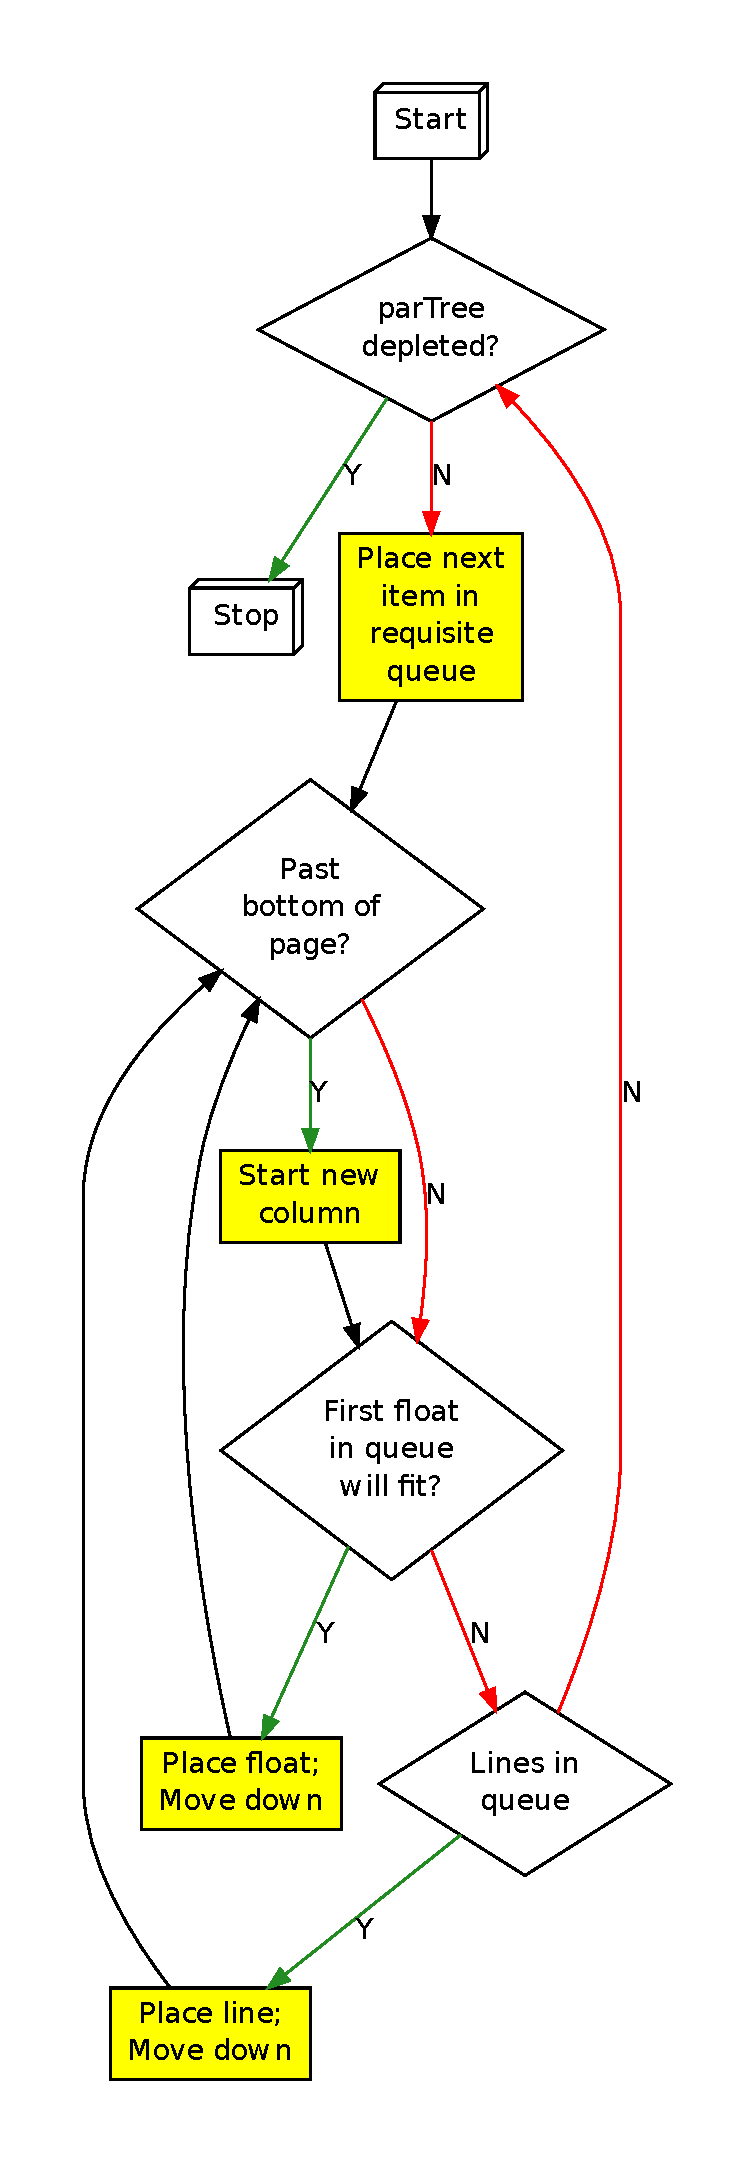
\includegraphics[height=\textheight]{gfx/floatqueueflowchart}
  \end{center}
  \caption[Flowchart of the two-queue float algorithm]{Flowchart describing the two-queue float algorithm}
  \label{fig:float-flowchart}
\end{figure}

Pagination is reasonably simple with this queueing system: as soon as a page is full, the layout can be restarted at the origin of the page using the current status of both queues and the document structure tree. It is entirely possible that floats may appear on pages subsequent to their callout point in the text, but this effect should be no worse than in many current typesetting systems.

While this approach does produce reasonable layouts, and handles floats well without the need for backtracking, it is not particularly conducive to producing layouts with floats that span multiple columns. The queue-based layout described above is rather simplistic: it knows about the size of each component that it lays out, but it does not remember the history of the positions of any of the components that are already laid out. This makes it difficult to have items that span more than one column, because there is no mechanism to mark space on the page as being reserved. In order to do this, another approach must be taken.

\subsection{A Grid-Based Layout}
% - Support of floats
    % - Queue system
    % - Grid/array system (no need for queue)
    % - Multicolumn floats
        % - issues with spanning \& pagination
A simple method for allowing parts of a page to be reserved is to break it up into a grid. Grid-based layouts are useful in many situations~\cite{Collier1991}; one example of particular note is that of modern-day newspapers (see figure~\ref{fig:gridlayout}). Following the example set by these newspapers, the grid used in this system is defined to have a row height of the \gls{leading} of the document's body text, and a column width of the \gls{measure} of one text column plus the required gutter space.

\begin{figure}
    \includegraphics[width=\textwidth]{gfx/newspaper}
    \caption[An example of a grid-based layout]{An example of a grid-based layout in a UK newspaper. Note how all the baselines of the main body text are aligned to a common grid, and that all items span integer multiples of columns.}
    \label{fig:gridlayout}
\end{figure}

The viewer uses the dimensions of the float, as specified in the document structure tree (see section \ref{sec:docgen}), to determine how many columns it should span. The float is scaled to span the integer multiple of column widths that most closely matches its `natural' size, though for reasons that should hopefully be obvious, this number is limited to a minimum of 1, and a maximum of the number of columns on the page. Additionally, checks are made to ensure that the scaling will not cause the height of the figure to exceed that of the page.

An advantage of this grid-based approach is that it no longer requires the use of queues, either for lines, or for floats. The viewer simply traverses the document structure tree, placing each item in the first available place in the grid. In the case of floats, or other items larger than multiples of the main \gls{leading}, spaces in the grid can be marked as reserved, to prevent other items from trampling over their reserved space. If a float will not fit directly below the previous item to be placed, the grid is walked over until a gap of sufficient size can be found. Figure~\ref{fig:screengrab} shows an example of a document laid out with this system.



\begin{figure}
    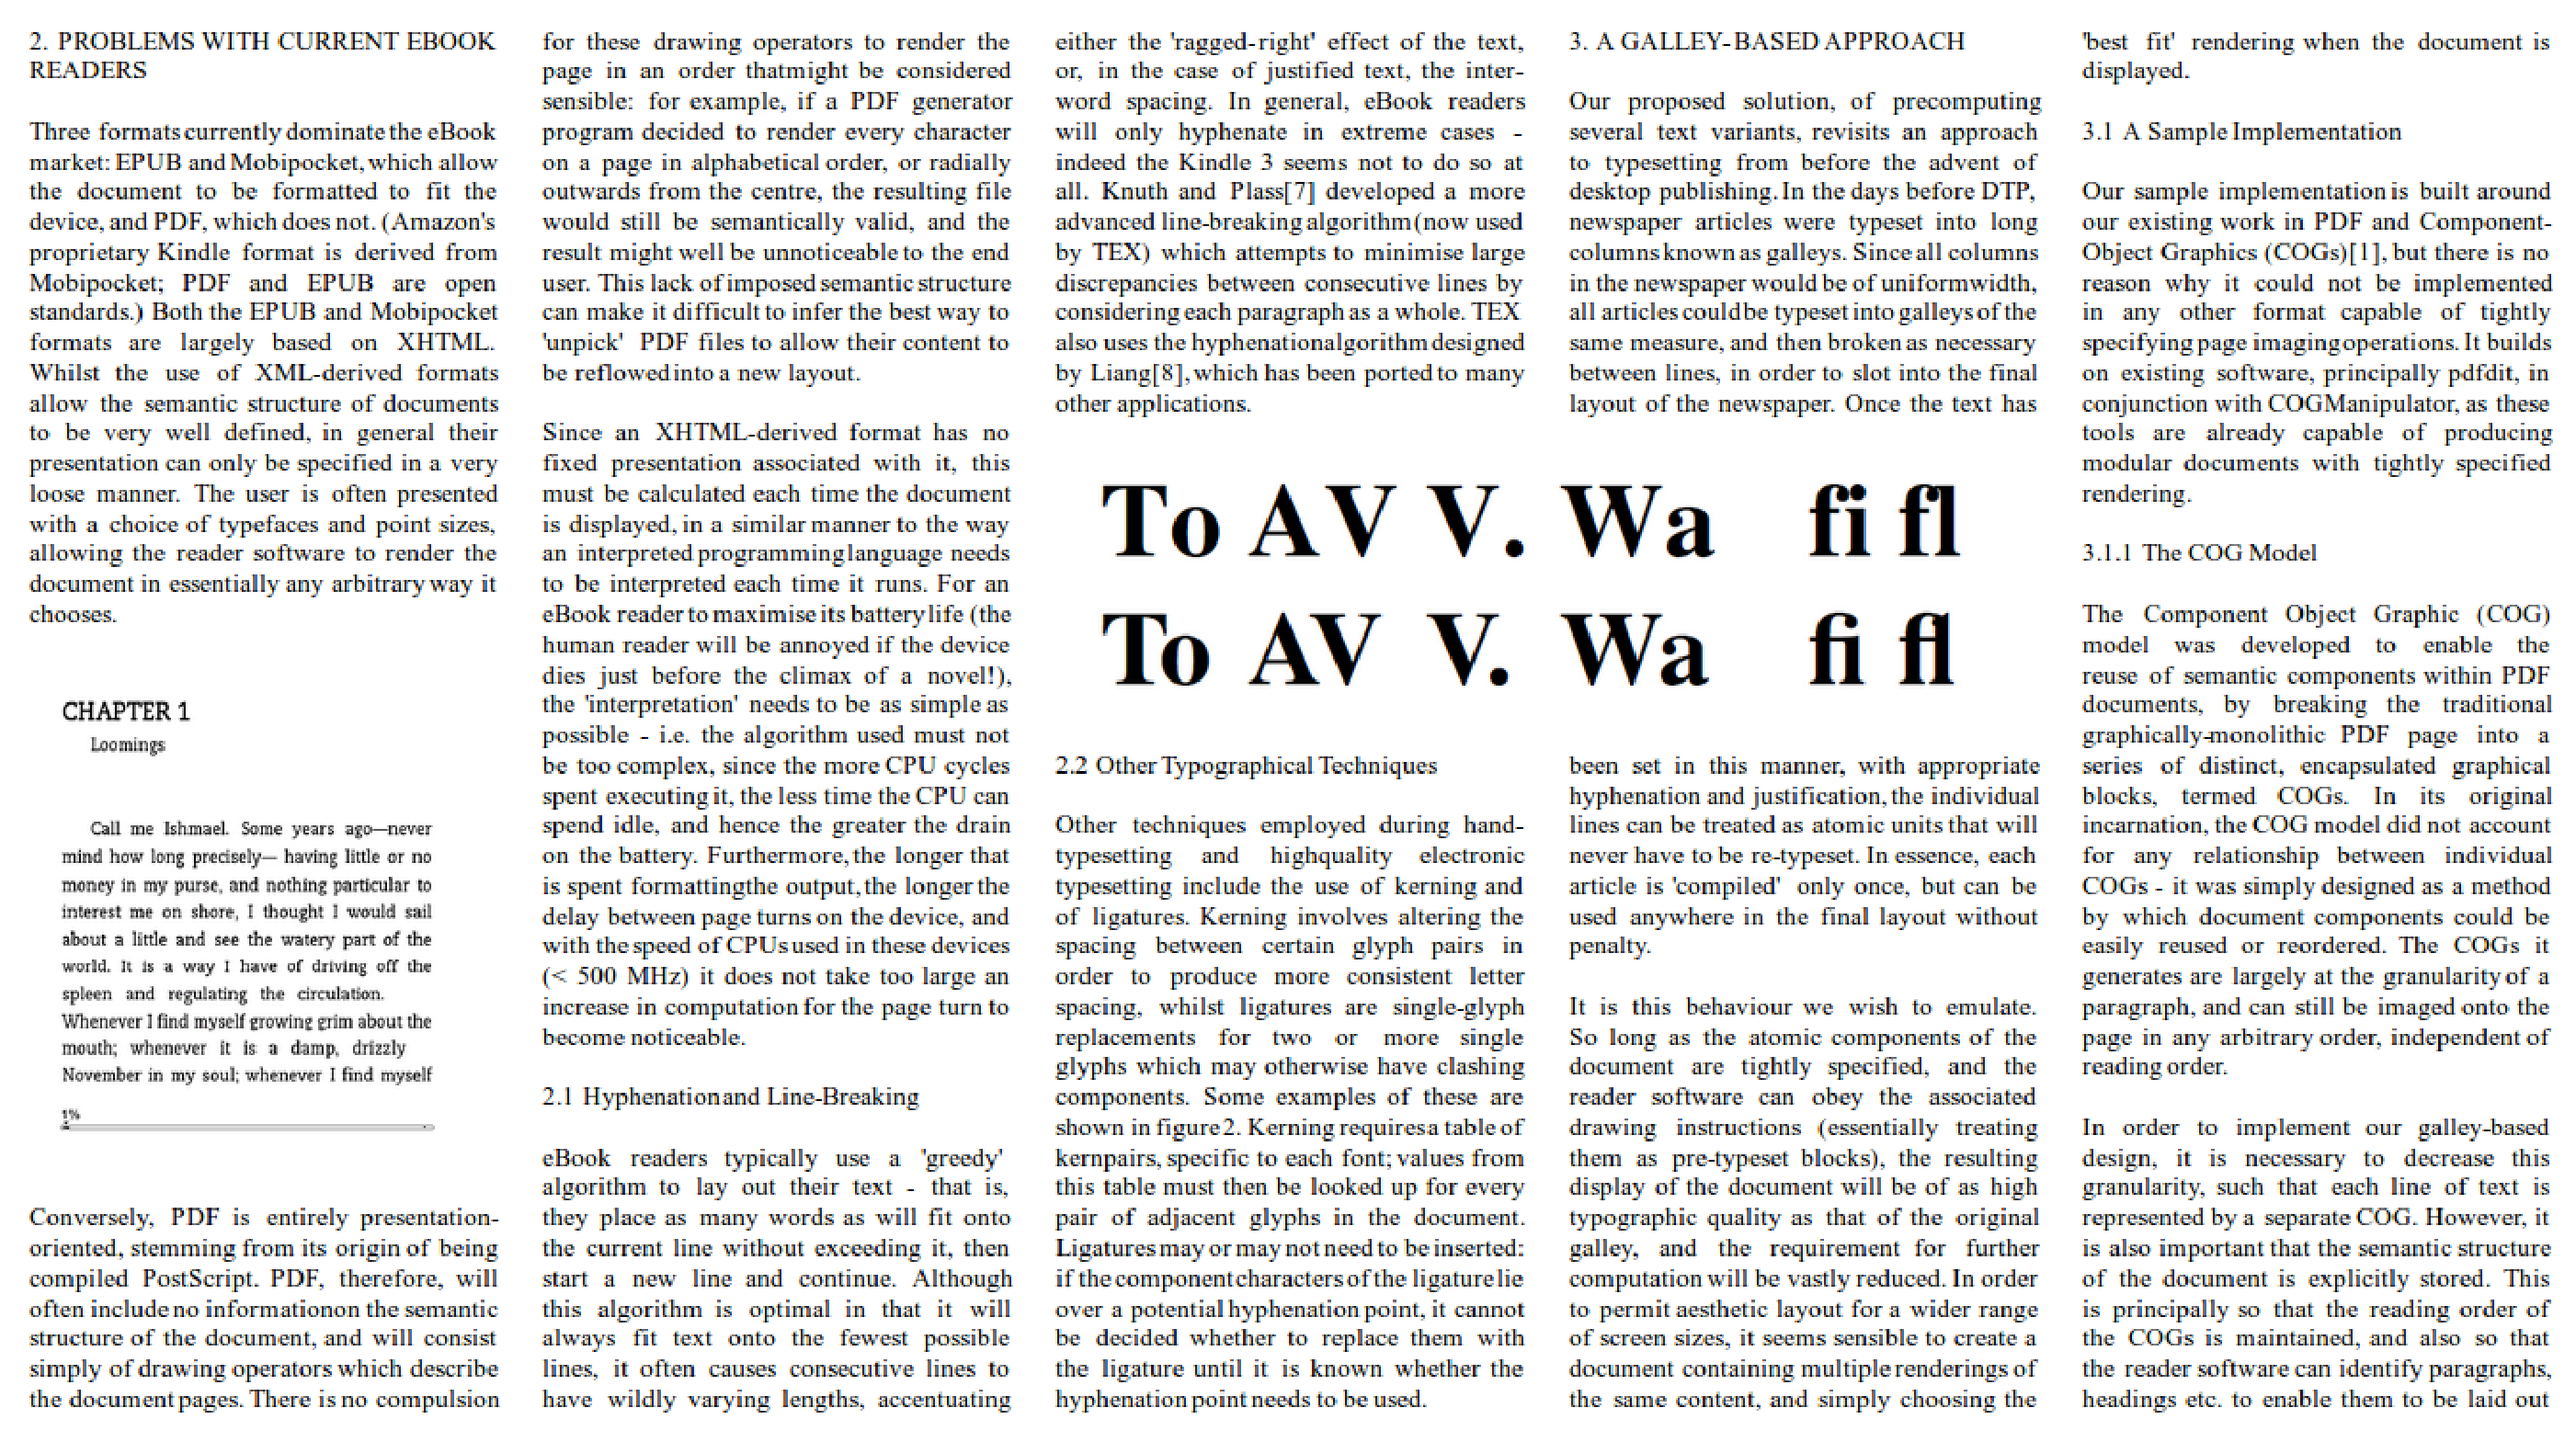
\includegraphics[angle=90,origin=c,width=\textwidth]{gfx/floatrendering}
    \caption[A sample rendering with multi-column floats]{An excerpt from \cite{Pinkney2011}, typeset and rendered by the system described in chapter~\ref{ch:floats}. Of the two floats (a screenshot from a Kindle, and a demonstration of some micro-typographical techniques), one spans only one column, and one spans two. }
    \label{fig:screengrab}
\end{figure}

Pagination becomes a little trickier when floats are allowed to span multiple columns. For example, if a float, whose natural size would lead it to span $n$ columns, is encountered in the document structure tree when there are $(n-1)$ or fewer columns remaining to be typeset on the page, it must be decided how best to handle the situation. Three obvious options present themselves: alter the float to span fewer columns; delay the placement of the float until the start of the next page; or backtrack and check whether there is room to move the float back one or more columns, by shunting non-floatable text lines forwards.

The first option is clearly not desirable behaviour, given that shrinking a float may well reduce its legibility. Additionally, if this becomes a common problem, it it likely to be noticeable that floats spanning into the rightmost column of the page appear shrunken. The second option (delaying placement until the following page) is a reasonable compromise, though it will increase float-drift (whereby floats become separated from their callout points in the text), which is not ideal. The third option (backtracking and shunting) is likely to produce the most desirable output, although some computational overhead will be added. One approach is simply to check whether there is enough space immediately to the left (specifically a gap between other, already placed, floats) into which the current float can be placed, with the displaced lines being shunted forwards. This method will not produce layouts as optimal as methods that use full backtracking and check all possibilities, but it will run in much quicker time. A combination of all three of the above options is likely to work best in practice.


% \todo{Actually implement some of these pagination schemes, and write something intelligent-sounding about it. Provide some example output (screenshots).}

\section{Summary}

The reimplementation of the system in \html{} is not without its pitfalls. One strong advantage of using \pdf{} over \html{} is that any \pdf{} reader that correctly implements the standard~\cite{Adobe2001} should display any given document in an identical manner to any other reader. Regrettably (and much to the chagrin of web developers everywhere) this is very much not true of rival web browser layout engines. Though standards do exist (published by the \gls{w3c}) and are largely adhered to by all the major layout engines, there are certain areas that are open to interpretation by the developers. One particular problem that is encountered when using the system described in this chapter is that of font scaling. The layouts produced by this system will only retain its quality if it is laid out precisely as specified by the typesetting process. Viewing the malleable documents in Google Chrome and Mozilla Firefox (which use WebKit and Gecko respectively) produces noticeably different results when the user chooses to scale the page up: WebKit appears to be inconsistent and non-linear when scaling fonts, whereas Gecko does a better job, and manages to lay out the text as intended by the typesetter. Figure~\ref{fig:craprenderer} shows an example of Gecko's font scaling problem.

\begin{figure}
    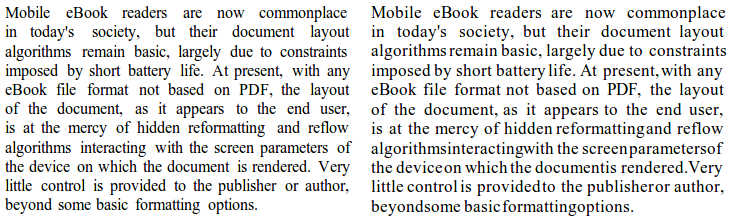
\includegraphics[width=\textwidth]{gfx/webkitisshit}
    \caption[Inconsistent font scaling by WebKit]{Chrome and Safari's layout engine (WebKit) can be inconsistent when scaling fonts. The paragraph to the left is displayed ``correctly'', but the paragraph to the right (scaled up by 1\% by the JavaScript) has clearly not scaled linearly. In contrast, Firefox's layout engine, Gecko, scales smoothly, and behaves as one might expect when zooming in on a \pdf{} file, which was the intended behaviour.}
    \label{fig:craprenderer}
\end{figure}



\todo{Write some analysis of the various float algorithms; provide some criticism of growing file sizes which leads onto the next chapter; mention problems that occur when the renderer tries to be clever (eg does its own kerning) ie Webkit vs Gecko}
\chapter{Dealing with File Bloat}\label{ch:bloat}
\redmarginpar{Have done the groundwork for this chapter (results in table~\ref{tab:filesize}) but need to do some more on comparing different compression schemes, and then write about it.}

\section{Rationale}
In the system thus far described in this thesis, the emphasis has been firmly upon reducing the computational complexity of layout operations at view-time of a document, and therefore little consideration has been given to the filesize of the resultant malleable documents.

\todo{Put in some pdfdump output comparing ``normal'' pdfs with my malleable ones (maybe as an appendix)}

The resultant tradeoff between filesize and required computation has previously been justified on the basis that storage is both cheap (as of 2013 one US dollar will buy around two gigabytes of \textsc{nand} flash memory) and light; and batteries, although not enormously expensive either, already comprise a significant proportion of the overall mass of most portable devices suitable for reading \ebook{}s. The upshot is that adding more storage to a device has little impact upon devices' aesthetics, but that adding extra battery life (emerging nanotube battery technology notwithstanding) would result in vast increases in the devices' overall bulk and mass.

Despite this, it seems perverse to make no attempt at all to keep filesizes as small as possible, as long as there are no (or limited) impacts upon the required computation at view-time.

\section{Implementation}
The most obvious saving that can be made is with the duplication of a document's textual content. The systems described in chapters \ref{ch:malleable}~and~\ref{ch:floats} both contain as many copies of the document text as there are pre-rendered galleys; in practice, though, there is no real need for more than one copy to be present in the file. Two approaches to this problem were considered.

\subsection{Pointers into the Source Text}
The first approach to be considered was to include the source text of the document in its entirety, and for each rendering to contain only pointers to the relevant sections of text, instead of the words themselves. These pointers can either be physical\redmarginpar{I don't think ``physical'' is the right word here. What is???} (in the form of a character offset from the start of the text) or logical (in the form \emph{paragraph m, word n}). If the document text is to be included as a plaintext string, physical pointers are easier to use than logical: logical pointers either require an auxiliary data structure to map the logical pointers to physical ones, or for the document text to be stored in a format reflecting the logical structure, \ie{} not in plain text.

A drawback of using this approach is that on occasion, the output of the linebreaking process does not exactly match the input: for example in the case where words are hyphenated (requiring one word to be broken into two parts, and the addition of a hyphen) or where certain glyphs may be substituted for others (such as with the use of ligatures, where a glyph pair or triplet may be replaced with a single glyph).



\subsection{Use of a Dictionary}
The second approach considered was the use of a \emph{dictionary} (or \emph{map}) to act as a lookup table for each word-level item produced by the linebreaking process.

\begin{figure}
  \begin{center}
  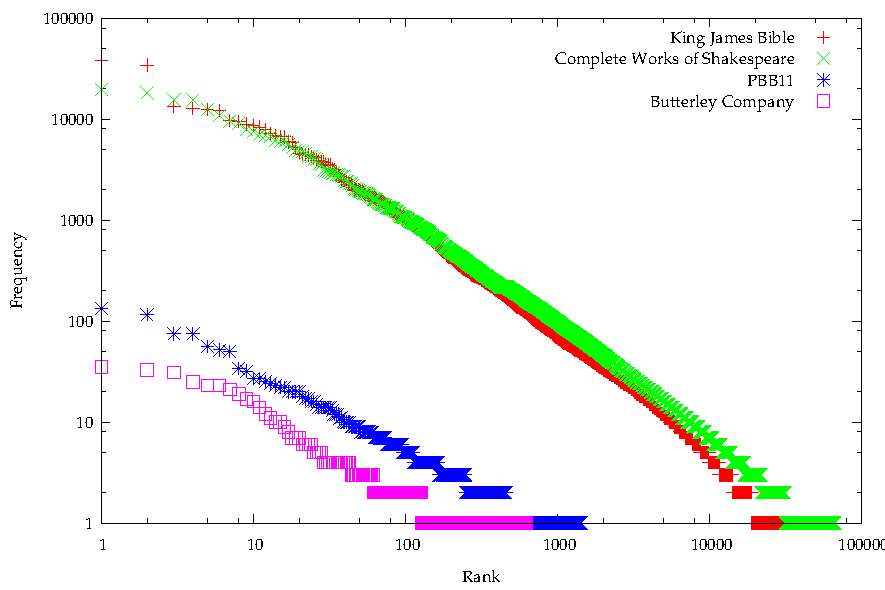
\includegraphics[width=\textwidth]{gfx/wordfreq}
  \end{center}
  \caption[Word frequencies in various documents]{Word frequencies in various documents, plotted on a log-log scale. All of these documents, despite their varying lengths, appear to conform well with Zipf's Law. }
  \label{fig:wordfreq}
\end{figure}

If, for example, if the word ``shall'' appears several times in a document (in the King James Version of the Bible it appears 9760 times, and in the complete works of Shakespeare 3016 times) it is only stored once in the dictionary. As long as a word's key is lexicographically shorter than the word itself, it can be guaranteed that some redundancy has been removed from the data.


\section{Results}

\subsection{Ordered dictionary with absolute positioning}

\begin{figure}
  \begin{center}
  \includegraphics[width=\textwidth]{gfx/scaling}
  \end{center}
  \caption[Filesize versus number of renderings, using absolute positioning]{Filesize in bytes, for a selection of documents that contain varying numbers of galley renderings, using an ordered dictionary and absolute positioning}
  \label{fig:sizescale}
\end{figure}

\begin{figure}
  \begin{center}
  \includegraphics[width=\textwidth]{gfx/scalingpersrc}
  \end{center}
  \caption[Filesize as a proportion of source document size, versus number of renderings, using absolute positioning]{Filesize as a proportion of source document filesize, for a selection of documents that contain varying numbers of galley renderings, using an ordered dictionary and absolute positioning}
  \label{fig:sizescalepersrc}
\end{figure}

\begin{figure}
  \begin{center}
  \includegraphics[width=\textwidth]{gfx/scalingpersrcpern}
  \end{center}
  \caption[Filesize as a proportion of source document size, per rendering, versus number of renderings, using absolute positioning]{Filesize as a proportion of source document filesize and per galley rendering, for a selection of documents that contain varying numbers of galley renderings, using an ordered dictionary and absolute positioning}
  \label{fig:sizescalepersrcpern}
\end{figure}


\subsection{Ordered dictionary with relative positioning}

\begin{figure}
  \begin{center}
  \includegraphics[width=\textwidth]{gfx/scalingdeltas}
  \end{center}
  \caption[Filesize versus number of renderings, using relative positioning]{Filesize in bytes, for a selection of documents that contain varying numbers of galley renderings, using an ordered dictionary and relative positioning, with word widths stored in the dictionary}
  \label{fig:sizescaledeltas}
\end{figure}

\begin{figure}
  \begin{center}
  \includegraphics[width=\textwidth]{gfx/scalingdeltaspersrc}
  \end{center}
  \caption[Filesize as a proportion of source document size, versus number of renderings, using relative positioning]{Filesize as a proportion of source document filesize, for a selection of documents that contain varying numbers of galley renderings, using an ordered dictionary and relative positioning, with word widths stored in the dictionary}
  \label{fig:sizescaledeltaspersrc}
\end{figure}

\begin{figure}
  \begin{center}
  \includegraphics[width=\textwidth]{gfx/scalingdeltaspersrcpern}
  \end{center}
  \caption[Filesize as a proportion of source document size, per rendering, versus number of renderings, using relative positioning]{Filesize as a proportion of source document filesize and per galley rendering, for a selection of documents that contain varying numbers of galley renderings, using an ordered dictionary and relative positioning, with word widths stored in the dictionary}
  \label{fig:sizescaledeltaspersrcpern}
\end{figure}

\begin{table}
    \myfloatalign
  \begin{tabularx}{\textwidth}{lXXXXXX} %\toprule
    & \multicolumn{2}{l}{\textsc{source text}} & \multicolumn{2}{l}{\textsc{orig. scheme}} & \multicolumn{2}{l}{\textsc{dictionary}} \\
    & \textsc{plain} & \textsc{gz} & \textsc{plain} & \textsc{gz} & \textsc{plain} & \textsc{gz} \\ \midrule
    PBB11~\cite{Pinkney2011} & 23\textsc{k} & 9.4\textsc{k} & 627\textsc{k} & 145\textsc{k} & 314\textsc{k} & 111\textsc{k} \\ \midrule
    King James Bible & 4.3\textsc{m} & 1.4\textsc{m} & 144\textsc{m} & 32\textsc{m} & 73\textsc{m} & 24\textsc{m} \\ 
    \bottomrule
  \end{tabularx}
  \caption[Comparison of filesizes]{Comparison of filesizes using various encoding methods}  \label{tab:filesize}
\end{table}
\chapter{Galley Generation Techniques}\label{ch:galleys}


(Is there a whole chapter's worth here?)

\begin{itemize}
 \item trying to match line breaks to make different widths swappable
 \item allow words to be placed separately (or have spacing altered) for extreme edge cases?
\end{itemize}



\chapter{Performance and Problems}\label{ch:perf}



\chapter{Conclusions, Evaluation, and Future Work}\label{ch:conclusions}


The system described in chapter~\ref{ch:floats} has only very basic support for floats. A particular limitation is that unlike paragraphs, each float has only one rendering, which must be scaled up or down as required, to fit across multiples of columns. Whilst for image-based figures or illustrations, this is probably already the desired behaviour, other types of floats, such as tables or code listings, would almost certainly benefit from the inclusion of multiple width renderings, with the choice of which rendering to display to be made at view-time. % Say that these could be differing hand-renderings, or automated from some source? Probably don't need to...

% coordinating breakpoints? might leave this until I have something sensible to say

Since the malleable document and viewer are composed entirely from HTML, CSS, and JavaScript\ed the core technologies behind EPUB\,---\,modifying the system to produce self-contained EPUB files seems an obvious next step.

%%%%%%%%%%%%%%%%%%%%%%%%%%%%%%%%%%%%%%%%%%%%%%%%%%
\singlespacing

% ********************************************************************
% Backmatter
%*******************************************************
\appendix
\cleardoublepage
%\part{Appendix}

%%********************************************************************
% Appendix
%*******************************************************
% If problems with the headers: get headings in appendix etc. right
%\markboth{\spacedlowsmallcaps{Appendix}}{\spacedlowsmallcaps{Appendix}}
\chapter{Source Code Listings}


\section{Java Paragraph Splitter}
\label{app:parsplitter}
\subsection{ParSplitter.java}
\lstinputlisting[nolol,language=Java,tabsize=4,stringstyle=\color{blue},basicstyle=\ttfamily\scriptsize]{../../../../public_html/JSReflow/ParSplitter/src/ParSplitter.java}

\newpage

\section{C Linebreaker}
\label{app:linebreaker}
\subsection{main.c}
\lstinputlisting[nolol,language=c,tabsize=4,stringstyle=\color{blue},basicstyle=\ttfamily\scriptsize]{../../../../public_html/JSReflow/LineBreak/main.c}

\newpage

\subsection{Formatter.h}
\lstinputlisting[nolol,language=c,tabsize=4,stringstyle=\color{blue},basicstyle=\ttfamily\scriptsize]{../../../../public_html/JSReflow/LineBreak/Formatter.h}

\newpage

\subsection{Formatter.c}
\lstinputlisting[nolol,language=c,tabsize=4,stringstyle=\color{blue},basicstyle=\ttfamily\scriptsize]{../../../../public_html/JSReflow/LineBreak/Formatter.c}

\newpage

\subsection{parseAFM.h}
\lstinputlisting[nolol,language=c,tabsize=4,stringstyle=\color{blue},basicstyle=\ttfamily\scriptsize]{../../../../public_html/JSReflow/LineBreak/parseAFM.h}

\newpage

\subsection{parseAFM.c}
\lstinputlisting[nolol,language=c,tabsize=4,stringstyle=\color{blue},basicstyle=\ttfamily\scriptsize]{../../../../public_html/JSReflow/LineBreak/parseAFM.c}

\newpage

\section{A Sample Malleable Document}
\label{app:sampledoc}
\subsection{butterley.html}
\lstinputlisting[nolol,language=html,tabsize=4,stringstyle=\color{blue},basicstyle=\ttfamily\scriptsize]{../../../../public_html/JSReflow/butterley.html}

\subsection{style.css}
\lstinputlisting[nolol,tabsize=4,stringstyle=\color{blue},basicstyle=\ttfamily\scriptsize]{../../../../public_html/JSReflow/styles.css}
\newpage

\subsection{script-json.js}
\lstinputlisting[nolol,language=c,tabsize=4,stringstyle=\color{blue},basicstyle=\ttfamily\scriptsize]{../../../../public_html/JSReflow/script-json.js}

\newpage

\subsection{butterley.js}
\lstinputlisting[nolol,language=c,tabsize=4,stringstyle=\color{blue},basicstyle=\ttfamily\scriptsize]{../../../../public_html/JSReflow/butterley.js}

%********************************************************************
% Other Stuff in the Back
%*******************************************************
\printglossaries
\newpage
%********************************************************************
% Bibliography
%*******************************************************
% work-around to have small caps also here in the headline
\manualmark
\markboth{\spacedlowsmallcaps{\bibname}}{\spacedlowsmallcaps{\bibname}} % work-around to have small caps also
%\phantomsection 
\refstepcounter{dummy}
\addtocontents{toc}{\protect\vspace{\beforebibskip}} % to have the bib a bit from the rest in the toc
\addcontentsline{toc}{chapter}{\tocEntry{\bibname}}
\bibliographystyle{plainnat}
\label{app:bibliography} 
\bibliography{refs}
\cleardoublepage
\pagestyle{empty}

\hfill

\vfill


\pdfbookmark[0]{Colophon}{colophon}
\section*{Colophon}
This document was typeset using the typographical look-and-feel \texttt{classicthesis} developed by Andr\'e Miede. 
The style was inspired by Robert Bringhurst's seminal book on typography ``\emph{The Elements of Typographic Style}''. \cite{Bringhurst2008}
\texttt{classicthesis} is available for both \LaTeX\ and \mLyX: 
\begin{center}
\url{http://code.google.com/p/classicthesis/}
\end{center}
Happy users of \texttt{classicthesis} usually send a real postcard to the author, a collection of postcards received so far is featured here: 
\begin{center}
\url{http://postcards.miede.de/}
\end{center}
 
\bigskip

\noindent\finalVersionString






%*******************************************************
% Declaration
%*******************************************************
\refstepcounter{dummy}
\pdfbookmark[0]{Declaration}{declaration}
\chapter*{Declaration}
\thispagestyle{empty}
Put your declaration here.
\bigskip
 
\noindent\textit{\myLocation, \myTime}

\smallskip

\begin{flushright}
    \begin{tabular}{m{5cm}}
        \\ \hline
        \centering\myName \\
    \end{tabular}
\end{flushright}

% ********************************************************************
% Game Over: Restore, Restart, or Quit?
%*******************************************************
\end{document}
% ********************************************************************


% **************************************************************************************************************
% A Classic Thesis Style
% An Homage to The Elements of Typographic Style
%
% Copyright (C) 2011 Andr\'e Miede http://www.miede.de
%
% If you like the style then I would appreciate a postcard. My address 
% can be found in the file ClassicThesis.pdf. A collection of the 
% postcards I received so far is available online at 
% http://postcards.miede.de
%
% License:
% This program is free software; you can redistribute it and/or modify
% it under the terms of the GNU General Public License as published by
% the Free Software Foundation; either version 2 of the License, or
% (at your option) any later version.
%
% This program is distributed in the hope that it will be useful,
% but WITHOUT ANY WARRANTY; without even the implied warranty of
% MERCHANTABILITY or FITNESS FOR A PARTICULAR PURPOSE.  See the
% GNU General Public License for more details.
%
% You should have received a copy of the GNU General Public License
% along with this program; see the file COPYING.  If not, write to
% the Free Software Foundation, Inc., 59 Temple Place - Suite 330,
% Boston, MA 02111-1307, USA.
%
% **************************************************************************************************************
% Note:
%    * You must not use "u etc. in strings/commands that will be spaced out (use \"u or real umlauts instead)
%    * New enumeration (small caps): \begin{aenumerate} \end{aenumerate}
%    * For margin notes: \marginpar or \graffito{}
%    * Do not use bold fonts in this style, it is designed around them
%    * Use tables as in the examples
%    * See classicthesis-preamble.sty for useful commands
% **************************************************************************************************************
% To Do:
%		 * [high] Check this out: http://www.golatex.de/koma-script-warnung-in-verbindung-mit-listings-package-t2058.html
%    * [medium] mathbb in section-titles/chapter-titles => disappears somehow in headlines!!!
% **************************************************************************************************************